\documentclass[12pt]{article}
\usepackage{amsmath,amssymb,amsthm,bm}
\usepackage{geometry,graphicx,subcaption,sidecap}
\geometry{margin = 1 in}
\usepackage{color}

% Continuous notation:
\newcommand{\gcon}{g}
\newcommand{\kcon}{k}
\newcommand{\fcon}{f}
\newcommand{\blurV}{\nu}	% Variance of Gaussian blur function

% Discrete notation:
\newcommand{\gdis}{\mathbf{g}}
\newcommand{\gnoise}{\widetilde{\mathbf{g}}}
\newcommand{\kdis}{\mathbf{k}}
\newcommand{\kmat}{K}	% Matrix K
\newcommand{\fdis}{\mathbf{f}}
\newcommand{\tdis}{\mathbf{t}}
\newcommand{\ddis}{\mathbf{d}}	% Differential operator
\newcommand{\trans}{\mathrm{T}}	% Matrix transpose
\newcommand{\ctrans}{*}	% Conjugate transpose
\newcommand{\trace}{\operatorname{trace}}	% Trace
\newcommand{\diag}{\operatorname{diag}}

% Regularization notation:
\newcommand{\regparam}{\lambda}
\newcommand{\R}{R_{\regparam}}	% Regularization matrix
\newcommand{\freg}{\fdis_{\regparam}}	% Regularized solution
\newcommand{\argmax}{\operatorname{arg\,max}} % Arg max
\newcommand{\argmin}{\operatorname{arg\,min}} % Arg min

% Filter function:
\newcommand{\filt}{\phi}

% Noise notation:
\newcommand{\noiseSD}{\sigma}	% Standard deviation
\newcommand{\noise}{\bm{\eta}}	% Noise vector
\newcommand{\Var}{\operatorname{Var}}	% Variance
\newcommand{\E}{\operatorname{E}}	% Expected value

% Singular values and vectors:
\newcommand{\singular}{s}	% Singular values
\newcommand{\LSV}{\mathbf{u}}	% Left singular vector
\newcommand{\RSV}{\mathbf{v}}	% Left singular vector

% UPRE derivation notation:
\newcommand{\PE}{\mathbf{p}_{\regparam}}	% Predictive error
\newcommand{\regres}{\mathbf{r}_{\regparam}}	% Regularized residual
\newcommand{\A}{A_{\regparam}}	% Influence matrix
\newcommand{\U}{U}	% UPRE functional

% GCV derivation notation:
\newcommand{\GCV}{G}	% GCV functional

% Discrepancy principle derivation notation:
\newcommand{\D}{D}	% Discrepancy principle functional
% Rosie's commands
\newcommand{\comment}[1]{\textcolor{red}{ \textbf{Comment}: #1}}
% Defining Trace Lemma
\newtheorem*{TL}{Trace Lemma}

\title{\underline{Regularization Parameter Estimation (1D)}}
\author{Michael Byrne}
\date{\today}

\begin{document}
\maketitle

\section{Introduction} \label{Introduction}
Given functions $\gcon(x)$ and $\kcon(x,t)$, a \textit{Fredholm equation of the first kind} can be stated as
\begin{equation}
	\gcon(x) = \int_a^b \kcon(x,t)\fcon(t)\:dt,
	\label{Eq_Con}
\end{equation}
where the function $\fcon$ is unknown. If the kernel $\kcon$ is of the form $\kcon(x,t) = \kcon(x-t)$, then the integral equation represents the continuous convolution $\gcon = \kcon * \fcon$ over the interval $[a,b]$, and the kernel is spatially invariant. Convolution is a smoothing operation: if $\kcon$ is integrable and $\fcon$ is bounded and locally integrable, then $\kcon * \fcon$ is a continuous function \cite{DebnathLokenath1999ItHs}. In particular, if $\kcon$ and $\fcon$ are at least piecewise smooth and bounded, the resulting convolution $\kcon * \fcon$ is continuous. \par
If $\kcon * \fcon$ is considered a smoothing operation, then finding $\fcon$ such that $\gcon = \kcon * \fcon$, given $\gcon$ and $\kcon$, could be considered a ``sharpening" operation. For instance, consider the kernel $\kcon(t) = \exp(-200(t-\frac{1}{2})^2)$ and the piecewise-smooth function $\fcon(t)$ defined as:
\begin{equation}
\fcon(t) = \begin{cases}
\sin\left(8\pi{t}\right), & 0 < t \leq \frac{1}{4} \\
0, & \frac{1}{4} < t \leq \frac{1}{3} \\
24\left(t-\frac{1}{3}\right), & \frac{1}{3} < t \leq \frac{3}{8} \\
1, & \frac{3}{8} < t \leq \frac{5}{8} \\
-24\left(t-\frac{2}{3}\right), & \frac{5}{8} < t \leq \frac{2}{3} \\
0, & \frac{2}{3} < t \leq \frac{3}{4} \\
\sin\left(8\pi\left(t-\frac{3}{4}\right)\right), & \frac{3}{4} < t \leq 1
\end{cases}.
\label{Eq_TF2}
\end{equation}
The kernel $\kcon$ is smooth and bounded on $[0,1]$, and the function $\fcon$ is 1-periodic and bounded. Plots of $\fcon(t)$ and $\kcon(t)$ are shown in Figure \ref{FunctionKernelPlot}. \par
The kernel $\kcon(t) = \exp(-200(t-\frac{1}{2})^2)$ is an example of a Gaussian kernel. The form of a Gaussian kernel comes from the probability density function of the Gaussian distribution,
\[p(t) = \frac{1}{\sqrt{2\pi\blurV}}\exp\left(\frac{-(t-\mu)^2}{2\blurV}\right),\]
where $\mu$ is the mean and $\blurV$ is the variance. The mean is the center of the Gaussian distribution, as well as the abscissa of the absolute maximum. The variance is a measure of dispersion of the distribution; as $\blurV$ increases, the width of the graph of $p(t)$ increases. The standard deviation $\sqrt{\blurV}$ is also a measure of dispersion, though variance will be the measure of choice in this report. The scale factor $1/\sqrt{2\pi\blurV}$ ensures that $\int_{\mathbb{R}} p(t) \: dt = 1$, an essential property of a continuous probability distribution defined on the entire real line. For Gaussian kernels, however, this scale factor may be dropped since having a unitary integral is not required of kernels in general.  For the Gaussian kernel example $\kcon(t) = \exp(-200(t-\frac{1}{2})^2)$, the mean is 1/2 and $-200 = -1/2\noiseSD$ implies that $\blurV = 1/400$. Figure \ref{GaussianDistributions} illustrates the relationship between variance and width of the Gaussian distribution. It should be noted that the choice of $\blurV$ as the symbol for variance of the Gaussian distribution is nonstandard; a common choice for this variance is $\sigma^2$, though in this report $\sigma^2$ is reserved for the variance of the white noise from which $\noise$ is drawn in \eqref{Eq_DisNoise}. Another alternative for $\blurV$ would be $s^2$, though $s$ is reserved for singular values, the diagonal entries of $\Sigma$ in \eqref{Eq_SVD}. 

\begin{figure}
	\centerline{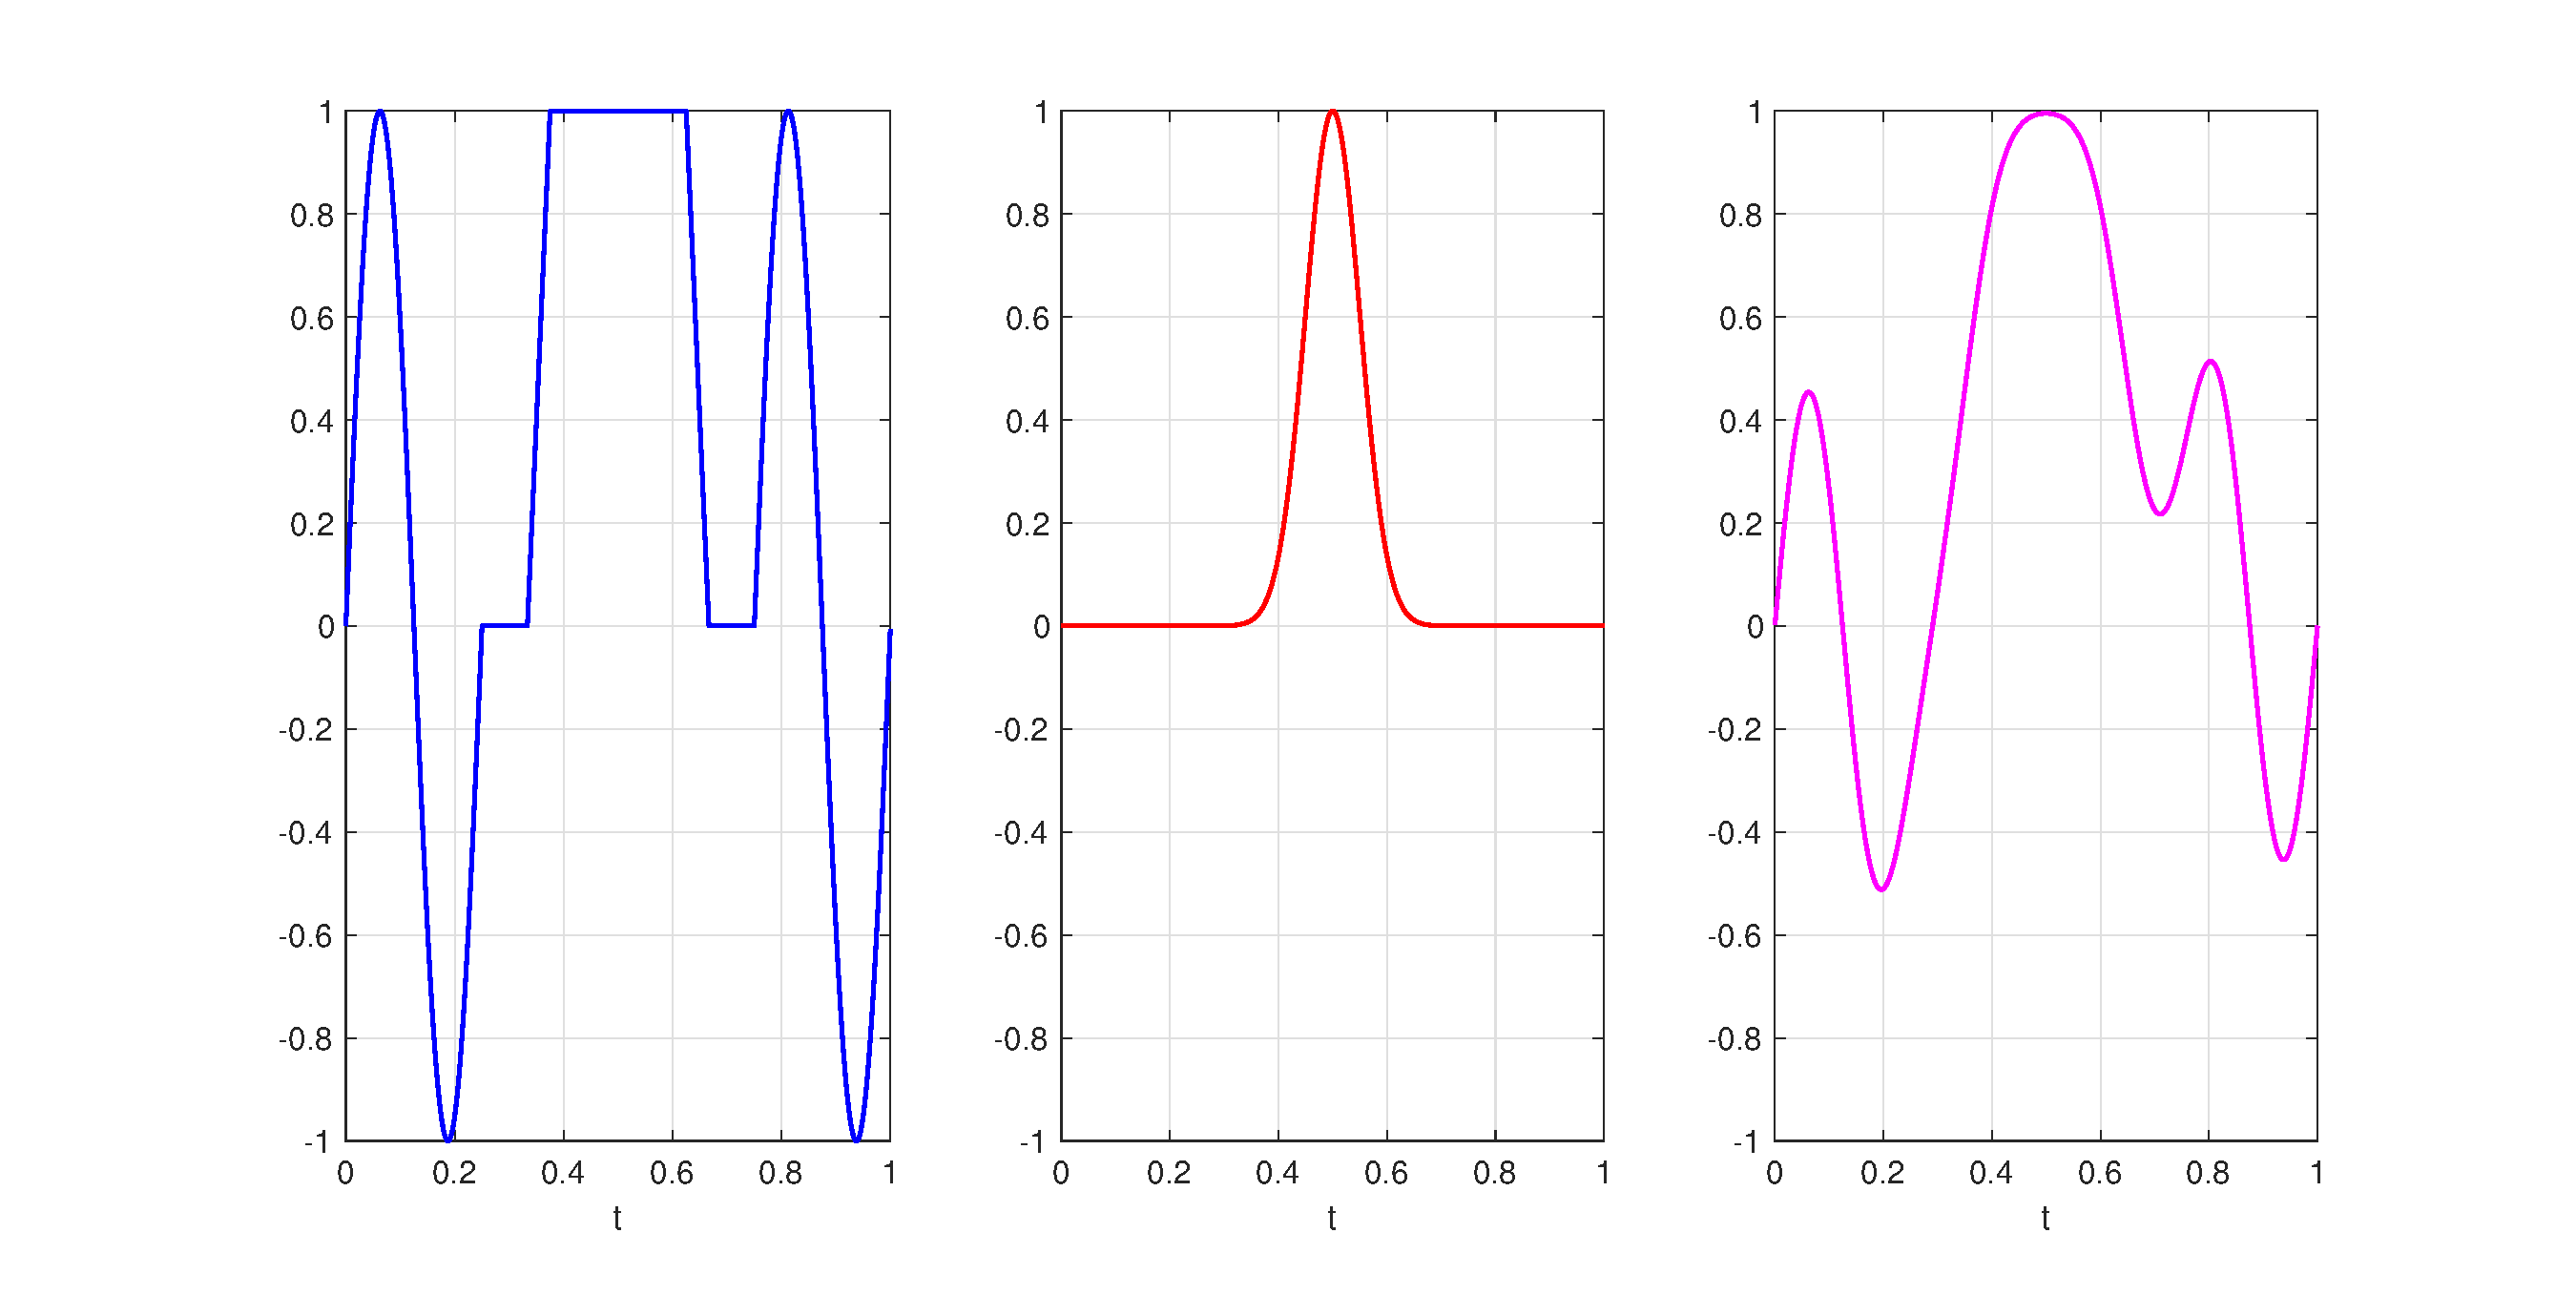
\includegraphics[scale=0.4]{Figures/FunctionKernelPlot.eps}}
\caption{Left: The graphs of the piecewise-smooth function $\fcon(t)$. Right: The Gaussian kernel $\kcon(t)$.}
\label{FunctionKernelPlot}
\end{figure}

\begin{figure}
	\centerline{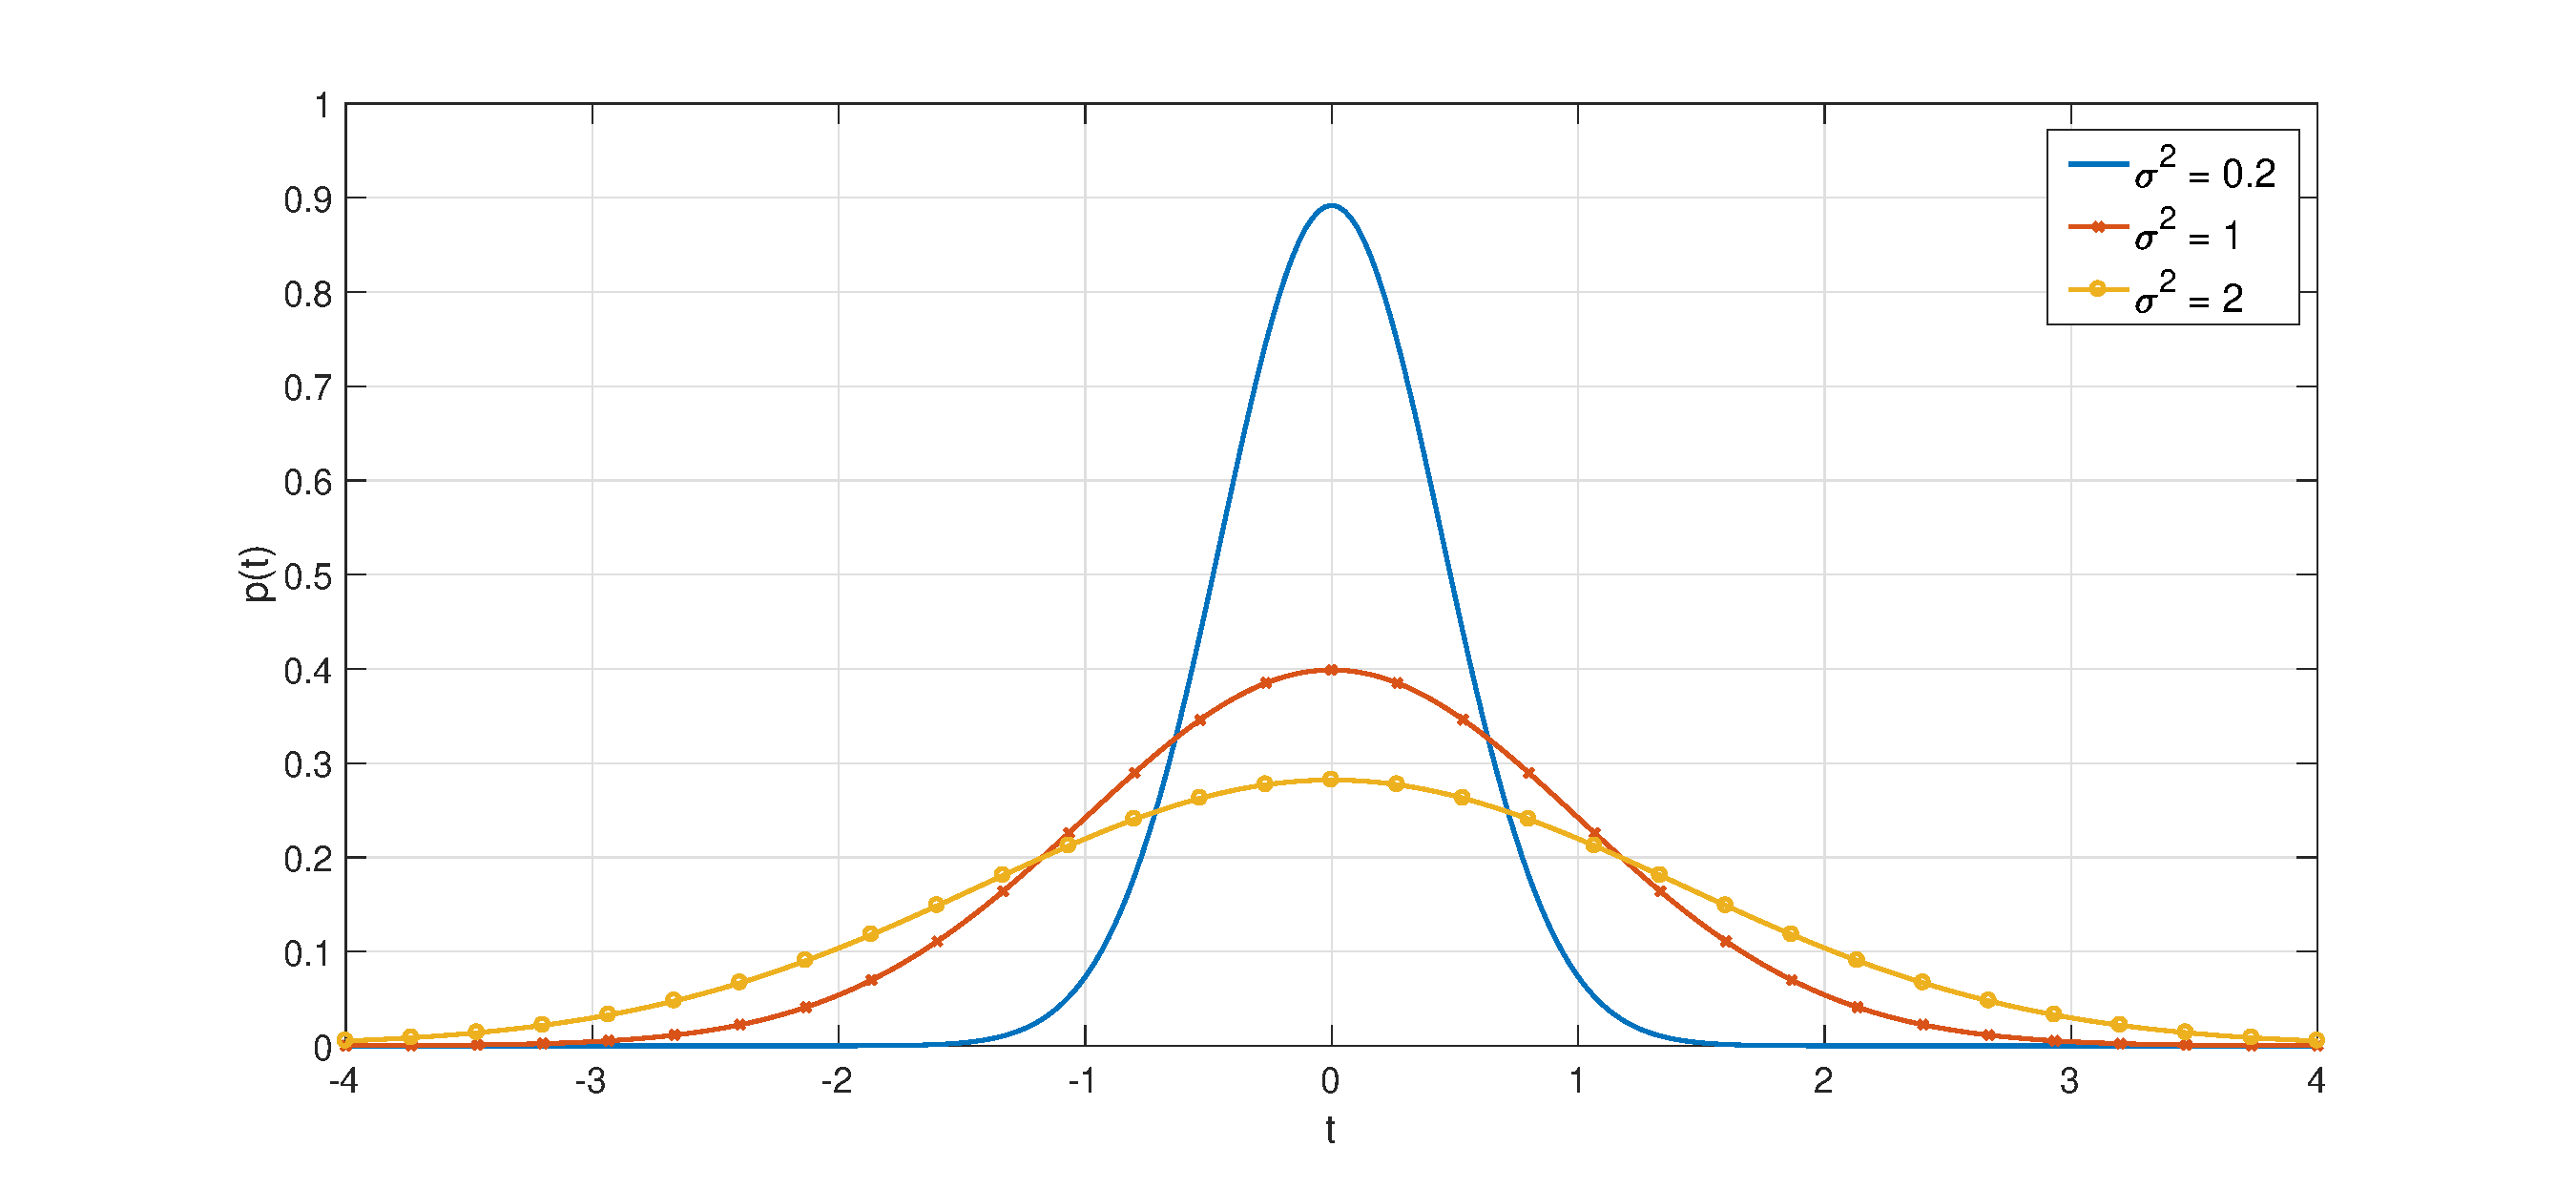
\includegraphics[scale=0.4]{Figures/GaussianDistributions.eps}}
\caption{Gaussian distributions for difference values of variance $\blurV$, all centered at the origin ($\mu = 0$). As $\blurV$ increases, the width of the distribution increases.}
\label{GaussianDistributions}
\end{figure}

To find a solution to the forward problem, which is the evaluation of $\gcon = \kcon * \fcon$, a quadrature method can be used to find a numerical approximation to the convolution integral. In the discrete setting, (1) can be stated as
\begin{equation}
\gdis = \kmat\fdis,
\label{Eq_Dis}
\end{equation}
where $\fdis$ and $\gdis$ are the vector discretization of $\fcon$ and $\gcon$, respectively, and $\kmat$ is a matrix representing the discrete convolution of $\kcon$ with $\fcon$. For example, suppose $\kcon(x,t)$ is a zero-centered Gaussian kernel and the domain of integration in \eqref{Eq_Con} is $[0,1]$. Given some $x_i \in [0,1]$, the continuous forward problem is to evaluate
\[g(x_i) = \int_0^1 \exp\left(\frac{-(x_i - t)^2}{2\blurV}\right)\fcon(t) \: dt.\]
If a left Riemann sum is used with $t_j = (j-1)/n$ for $j \in \{1,2,\ldots,n\}$, representing an equispaced discretization of $[0,1]$ using $n$ points, then
\[g(x_i) \approx \sum_{j=1}^n \frac{1}{n}\exp\left(\frac{-(x_i - t_j)^2}{2\blurV}\right)\fcon(t_j).\]
For approximations to $\gcon(x)$ at the same points that make up the equispaced discretization of $[0,1]$, i.e. at the points $x_i = (i-1)/n$ for $j \in \{1,2,\ldots,n\}$, then \eqref{Eq_Dis} is exactly the system that provides these approximations with $\fdis = [\fcon(t_1),\fcon(t_2),\ldots,\fcon(t_n)]$, $\gdis = [\gcon(x_1),\gcon(x_2),\ldots,\gcon(x_n)]$, and the elements of $\kmat$ being
\[K_{ij} = \frac{1}{n}\exp\left(\frac{-(i - j)^2}{2\blurV}\right).\]
Note that taking the collocation and quadrature points as the same ensures that the matrix $\kmat$ is square. Changing the number of collocation points, or the quadrature method, can change $\kmat$ from square to rectangular. \par
If the matrix $\kmat$ is nonsingular, then the solution to the inverse problem of \eqref{Eq_Dis} is $\fdis = \kmat^{-1}\gdis$. As with many linear systems, however, direct matrix inversion is discouraged and usually impractical since the matrix $\kmat$ becomes increasingly ill-conditioned as the size of the system grows \cite{Vogel:2002}. Unfortunately, large systems are necessary to adequately approximate the continuous problem, and so other methods of solving for $\fdis$ must be considered. \par
Before discussing the consequences of ill-conditioning, the concept of an well-posed problem will be introduced, which is due to Hadamard. Given an operator $A : \mathcal{H}_1 \rightarrow \mathcal{H}_2$, where $\mathcal{H}_1$ and $\mathcal{H}_1$ are Hilbert spaces, the equation $Af = g$ is said to be well-posed if
\begin{enumerate}
\item[(i)] for each $g \in \mathcal{H}_2$ there exists a solution $f \in \mathcal{H}_1$ to $Af = g$,
\item[(ii)] the solution $f$ is unique, and
\item[(iii)] if $Af_* = g_*$ and $Af = g$, then $f \rightarrow f_*$ whenever $g \rightarrow g_*$.
\end{enumerate}
In order, these conditions require that a solution exists, is unique, and is stable under perturbations in $g$. If one of these conditions is not met, then $Af = g$ is said to be an ill-posed problem. The discrete version $\kmat\fdis = \gdis$ of the problem in this report is ill-posed: singularity of $\kmat$ violates conditions (i) and (ii), and a poor condition number of nonsingular $\kmat$ violates condition (iii). This second case will now be discussed further.  \par 
A primary consequence of $\kmat$ being ill-conditioned relates to the accuracy of the vector $\gdis$. If $\gdis$ contains errors, as is often the case in practical applications, the errors are amplified during the multiplication $\kmat^{-1}\gdis$ since $\kmat$ is ill-conditioned and so the solution $\fdis$ will contain errors as well. For this consideration, the following system will be the assumed model throughout this report
\begin{equation}
\gnoise = \kmat\fdis + \noise
\label{Eq_DisNoise}
\end{equation}
where $\noise$ is a vector that represents any errors in $\gdis$ (this is equivalent to the statement $\gnoise = \gdis + \noise$). For further simplicity, assume that $\noise \sim \mathcal{N}(\bm{0},\noiseSD^2I)$, where $\bm{0}$ is the zero vector of length $n$ and $I$ is the $n \times n$ identity matrix. In other words, the error vector $\noise$ is an $n$-dimension Gaussian random variable with mean zero and variance $\noiseSD^2$. \par
Since direct matrix inversion is not practical, and at times not even possible since $\kmat$ can be singular, a singular value decomposition (SVD) of $\kmat$ can be an alternative. Assuming $\kmat$ is a real $m \times n$ matrix, the SVD of $\kmat$ is
\begin{equation}
\kmat = U\Sigma{V^\trans}
\label{Eq_SVD}
\end{equation}
where the $m \times m$ matrix $U$ and the $n \times n$ matrix $V$ have orthogonal columns and $\Sigma$ is a $m \times n$ diagonal matrix. The diagonal elements of $\Sigma$ are the singular values of $\kmat$, denoted $\singular_i$ and satisfying $\singular_1 \geq \singular_2 \geq \ldots \geq \singular_n \geq 0$. The columns of $U$ and $V$ will be denoted $\LSV_i$ and $\RSV_i$, respectively; these vectors are known as the left and right singular vectors of $\kmat$, respectively. A matrix of complex values has a SVD as well, the only difference being that the transpose is replaced with conjugate transpose. \par
Letting $r$ denote the rank of $\kmat$,  $\singular_1 \geq \ldots \geq \singular_r > 0$. In other words, the number of nonzero singular values of $\kmat$ is equal to the rank of $\kmat$.  A common variation of the SVD is the compact SVD, in which $\Sigma = \diag(\singular_1,\ldots,\singular_r)$, $U$ is an $m \times r$ matrix and $V^\trans$ is an $r \times n$ matrix. The matrices $U$ and $V$ are no longer orthogonal in the traditional sense because they are not square (unless $\kmat$ is nonsingular), though their columns remain orthonormal. For the remainder of this report all SVD's are assumed to be compact.  \par 
By using $\kmat^{-1} = V\Sigma^{-1}U^\trans$ when $\kmat$ is nonsingular, the product $\kmat^{-1}\gnoise$ is
\begin{equation}
\kmat^{-1}\gnoise = \kmat^{-1}\left(\kmat\fdis + \noise\right) = \fdis + \kmat^{-1}\noise = \fdis + V\Sigma^{-1}{U^\trans}\noise = \fdis + \sum_{i = 1}^n \frac{{\LSV^\trans_i}\noise}{\singular_i}\RSV_i. 
\label{Eq_InvProd}
\end{equation}
Even if $\kmat$ is singular, a solution can still be obtained by using the psuedoinverse $\kmat^+ = V{\Sigma^+}U^\trans$, where $\Sigma^+ = \diag(1/\singular_1,\ldots,1/\singular_r)$, and the upper bound of summation in \eqref{Eq_InvProd} becomes $r$. In either the nonsingular or singular case for $\kmat$, however, the summands in \eqref{Eq_InvProd} are numerically unstable for small $\singular_i$. For a visual representation of this instability, a Picard plot can be constructed. A Picard plot is a graph showing the terms $|\LSV^\trans_i\noise|/\singular_i$ in decreasing order with respect to the singular values. If the terms $|\LSV^\trans_i\noise|$ decay faster than $\singular_i$ as $i$ increases, then the terms $|\LSV^\trans_i\noise|/\singular_i$ do not become excessively large; this is the discrete Picard condition \cite{ABT}. The discrete Picard condition is thus a measure of instability. If the discrete Picard condition is not met, then the terms $|\LSV^\trans_i\noise|/\singular_i$ blow up as $i$ increases, often resulting in worthless solutions. In this experiment, the discrete Fourier transform will be used to obtain solutions analogous to those obtained by \eqref{Eq_InvProd}. In Section \ref{The Discrete Fourier Transform} a Picard plot is provided that demonstrates the relationship between the noise, the width of the Gaussian blur, and the resulting numerical instabilities related to obtaining meaningful solutions. See \cite{Hansen1990} for more information on Picard plots and the associated discrete Picard condition. \par 
A common approach to overcome numerical instabilities is to multiply the summands in \eqref{Eq_InvProd} by \textit{filter functions} $\filt$ that depend upon $\singular_i$ and a \textit{regularization parameter} $\regparam$. By doing so, an approximate solution is obtained:
\begin{equation}
\fdis(\regparam) = \sum_{i = 1}^n \RSV_i\filt(\regparam,\singular_i)\left(\frac{{\LSV^\trans_i}\gnoise}{\singular_i}\right).
\label{Eq_ApproxSol}
\end{equation}
The most desired property of the filter functions is that $\filt(\singular_i)/\singular_i \approx 1$  for large values of $\singular_i$ and $\filt(\singular_i)/\singular_i \approx 0$ for small values of $\singular_i$. A brief overview of common filter functions will now be provided. 

\subsection{Filter functions} \label{Filer functions}
Perhaps the simplest filter function is
\[\filt(\regparam,\singular_i) = \begin{cases}
1, & \singular_i^2 > \regparam \\
0, & \singular_i^2 \leq \regparam
\end{cases}\]
Using this function in (3) gives the approximate solution
\[\fdis(\regparam) = \sum_{\singular_i^2 > \regparam} \frac{{\LSV^\trans_i}\gnoise}{\singular_i}\RSV_i\]
which actually corresponds to the solution obtained using a truncated singular value decomposition (TSVD) of the matrix $\kmat$ \cite{Vogel:2002}. \par
A less simple filter function is
\begin{equation}
\filt(\regparam,\singular_i)  = \frac{\singular_i^2}{\singular_i^2 + \regparam}
\label{Eq_TikFilt}
\end{equation}
which is known as the Tikhonov filter function. For large values of $\regparam$, the above fraction is close to zero and for small values of $\regparam$, the fraction is near to unity. The use of the Tikhonov filter function to generate an approximate solution is known as \textit{Tikhonov regularization} \cite{Tikh1963}; the obtained solution is
\begin{equation}
\fdis(\regparam) = \sum_{i = 1}^n \filt(\regparam,\singular_i)\frac{{\LSV^\trans_i}\gnoise}{\singular_i}\RSV_i = \sum_{i = 1}^n \frac{\singular_i{\LSV^\trans_i}\gnoise}{\singular_i^2 + \regparam}\RSV_i.
\label{Eq_TikSol}
\end{equation}
An alternative representation of the above Tikhonov solution is
\begin{equation}
\fdis(\regparam) = \arg\min_{\fdis \in \mathbb{R}^n} \|\kmat\fdis - \gnoise\|^2 + \regparam\|D\fdis\|^2,
\end{equation}
where $D$ is the matrix representation of a linear operator. The term $\|D\fdis\|^2$ is commonly called the penalty function \cite{Vogel:2002}. The representation \eqref{Eq_TikSol} follows from selecting $D$ to be $I$, the $n \times n$ identity matrix. The kernel $k(x,t)$ and function $f(t)$ considered in Section \ref{Introduction} will be retained for the numerical examples included in this report.

\section{Analytical tools} \label{Analytical tools}

\subsection{Discrete convolution} \label{Discrete convolution}
As described in the Section \ref{Introduction}, the operation of convolution arises in various settings pertaining to inverse problems. Discrete convolution will first be described  in a general setting, followed by specific instances and connections to the numerical experiments conducted in this report. \par
Let $(x_n)$ and $(y_n)$ be sequences of complex numbers indexed by the integers. Then the discrete convolution of $(x_n)$ and $(y_n)$, denoted $x*y$, is defined by
\[(x*y)_n = \sum_{k=-\infty}^\infty x_{n-k}y_k.\]
The series in the definition of discrete convolution is bi-infinite, meaning that the discrete convolution might not be well-defined for any two arbitrary sequences. For example, if $x_n = y_n = 1$ for all $n \in \mathbb{Z}$, then the series defining $(x*y)_n$ is $\sum_{k=-\infty}^\infty 1$, which does not converge. In various cases, however, the discrete convolution is well-defined. These cases include sequences having only finitely-many nonzero terms and sequences in $\ell^1$. (In fact, the set of sequences having finitely-many nonzero terms is a linear subspace of $\ell^1$).  \par 
Fortunately, real-world applications usually involve finite sequences (vectors), which can be thought of as infinite or bi-infinite sequences having finitely-many nonzero terms. While such sequences do not require the evaluation of infinite series to compute discrete convolutions, it is helpful to have general results regarding the length and indices of discrete convolutions. Let $(x_n)$ and $(y_n)$ be nonzero sequences with finitely-many nonzero terms. For $(x_n)$, the assumptions imply the existence of integers $s_x$ and $e_x$ such that $x_n = 0$ for all $n \in \mathbb{Z}$ with either $n < s_x$ or $e_x < n$. Such integers exist for $(y_n)$ and will be denoted $s_y$ and $e_y$. The choice of letters reflects the fact that $s$ and $e$ represent the starting and ending indices of the section of the sequence where the terms can be nonzero. Extending this notation, the number of terms in this section of sequence is $n_x = e_x - s_x + 1$ and $n_y = e_y - s_y + 1$ for $(x_n)$ and $(y_n)$, respectively. From \cite{BoggessAlbert2001Afci}, the values of $s_{x*y}$, $e_{x*y}$, and $n_{x*y}$ are
\begin{align}
s_{x*y} &= s_x + s_y, \nonumber \\
e_{x*y} &= e_x + e_y, \label{Eq_ConResults} \\
n_{x*y} &= n_x + n_y - 1. \nonumber
\end{align}
As an illustrative example, let $\mathbf{x} = [1,2,3]$ and $\mathbf{y} = [4,5,6,7]$ be row vectors. The vectors can be thought of as the bi-infinite sequences $(x_n) = (\ldots,0,1,2,3,0\ldots)$ and $(y_n) = (\ldots,0,4,5,6,7,0,\ldots)$. If the sequences are indexed so that $x_1 = 1$ and $y_1 = 4$, then $s_x = s_y = 1$, $e_x = n_x = 3$, and $e_y = n_y = 4$. Then by \eqref{Eq_ConResults}, $s_{x*y} = 2$, $e_{x*y} = 8$, and $n_{x*y} = 6$. The bi-infinite sequence produced from the convolution is
\[x*y = (\ldots,0,4,13,28,34,32,21,0,\ldots),\]
where $(x*y)_2 = 4$ and $(x*y)_8 = 21$. \par 
Since the numerical experiments for this report are conducted in MATLAB, a brief remark regarding discrete convolutions in MATLAB will be given. If the built-in function \texttt{conv} is used to evaluate the discrete convolution of row vectors $\mathbf{x}$ and $\mathbf{y}$ described in the previous example, the output is the row vector $[4,13,28,34,32,21]$.  All vectors in MATLAB have a starting index of 1, and the vector resulting from the convolution is no different: the component 4 has an index of 1. While this seems to conflict with \eqref{Eq_ConResults} (recall that $s_{x*y} = 2$, not 1), from a practical standpoint there is little reason for concern; usually the components themselves are of interest and not the indexing of the bi-infinite sequence. If one wants to keep track of the indexing as the convolution is evaluated, index vectors can be defined for $\mathbf{x}$ and $\mathbf{y}$ and \eqref{Eq_ConResults} can be applied to obtain an index vector for the resulting convolution. See \cite{BoggessAlbert2001Afci} for an explicit MATLAB example. \par 

\subsection{Circulant matrices} \label{Circulant matrices}
In Section \ref{Discrete convolution}, the discrete convolution and some of its variants were discussed. In this section, matrices will be discussed that have connections to discrete convolutions and other concepts. \par 
The first type of matrix to be discussed is a \textit{Toeplitz matrix}. A matrix $T$ is called a Toeplitz matrix if it is constant along each diagonal. The following matrices are examples of Toeplitz matrices.
\[A = \begin{bmatrix}
1 & 2 \\
2 & 1 \\
3 & 2
\end{bmatrix}, \quad 
B = \begin{bmatrix}
1 & 2 & 3 \\
2 & 1 & 2 
\end{bmatrix}, \quad 
C = \begin{bmatrix}
1 &  2 \\
2 & 1
\end{bmatrix}.\]
It is important to notice that by definition, Toeplitz matices need not be square. \par 
The primary connection to be made in this report is that discrete convolutions can be described in the context of matrix-vector multiplication using Toeplitz matrices. For example, the discrete convolution of $\mathbf{x} = [1,2,3]$ and $\mathbf{y} = [4,5,6,7]$ from Section \ref{Discrete convolution} can be cast as a matrix-vector product by defining a matrix $X$ to be
\[X = \begin{bmatrix}
1 & 0 & 0 & 0 \\
2 & 1 & 0 & 0 \\
3 & 2 & 1 & 0 \\
0 & 3 & 2 & 1 \\
0 & 0 & 3 & 2 \\
0 & 0 & 0 & 3
\end{bmatrix}.\]
Certainly $X$ is a Toeplitz matrix, and $x*y$ can be expressed as $Xy^\trans$ with $x*y$ being a (column) vector of length $n_{x*y} = 6$; the length of this vector agrees with result \eqref{Eq_ConResults}. The operation $Xy^\trans$ is equivalent to \texttt{conv(x,y)} in MATLAB. \par 
If a matrix $C$ has the property that each row is the circular right shift of the components of the preceding row, then $C$ is called a \textit{circulant matrix}. The \textit{circular right shift} of a row vector $[x_1,x_2,\ldots,x_n]$ is $[x_n,x_1,\ldots,x_{n-1}]$. From this definition, every circulant matrix is also a Toeplitz matrix. Just like Toeplitz matrices, circulant matrices need not be square. For example,
\[C = \begin{bmatrix}
1 & 2 & 3 & 4 \\
4 & 1 & 2 & 3 \\
3 & 4 & 1 & 2
\end{bmatrix}\] 
is a circulant matrix generated by circular right shifts of the vector $[1,2,3,4]$. However, circulant matrices are often defined to be square, a convention that will be adopted in this report. Therefore every reference to circulant matrices from this point will be under the assumption that circulant matrices are square. A significant property of circulant matrices is that they are diagonalized by the discrete Fourier transform, a property that will be discussed in Section \ref{The Discrete Fourier Transform}.

\subsection{The Discrete Fourier Transform} \label{The Discrete Fourier Transform}
The \textit{discrete Fourier transform} (DFT) is a mapping $\mathcal{F}:\mathbb{C}^n \rightarrow \mathbb{C}^n$ defined by
\begin{equation}
\mathcal{F}(\mathbf{f})_j = \sum_{k=1}^{n} f_{k}\exp\left(\frac{-2\pi{ij}(k-1)}{n}\right), \quad \mathbf{f}\in\mathbb{C}^n,
\label{Eq_DFT}
\end{equation}
and $i = \sqrt{-1}$. The DFT of a vector $\mathbf{f}$ will be denoted by $\widehat{\mathbf{f}}$. The inverse DFT of a vector $\widehat{\mathbf{f}}$ is given by
\begin{equation}
\mathcal{F}^{-1}(\widehat{\mathbf{f}})_j = \frac{1}{n}\sum_{k=1}^{n} \widehat{f}_k\exp\left(\frac{2\pi{ij}(k-1)}{n}\right) = \mathbf{f}
\end{equation}
These definitions are slightly nonstandard in that the limits of summation are $k = 1$ to $n$, while the limits are using set to $k = 0$ and $n-1$; this is done to maintain the consistency of vector indexing. \par 
The DFT can also be stated in terms of matrix-vector multiplication. Given an $\mathbf{f} \in \mathbb{C}^n$, $\widehat{\mathbf{f}}$ can be expressed as $\widetilde{F}\mathbf{f}$ where the matrix $\widetilde{F}\in\mathbb{C}^{n\times{n}}$ has components
\[\widetilde{F}_{jk} = \exp\left(\frac{-2\pi{i(j-1)(k-1)}}{n}\right), \quad 1 \leq j,k \leq n.\] 
The matrix representing the inverse DFT is then $(1/n)\widetilde{F}^\ctrans$, where $\ctrans$ denotes conjugate transposition. Then since $(1/n)\widetilde{F}^\ctrans\widetilde{F} = (1/n)\widetilde{F}\widetilde{F}^\ctrans = I$, splitting the factor of $1/n$ as $(1/\sqrt{n})(1/\sqrt{n})$ allows for the Fourier matrix to be redefined as
\begin{equation}
F_{jk} = \frac{1}{\sqrt{n}}\exp\left(\frac{-2\pi{i(j-1)(k-1)}}{n}\right), \quad 1 \leq j,k \leq n
\label{Eq_DFT-Matrix}
\end{equation}
with the benefit being that $F$ is a unitary matrix: $F^\ctrans{F} = FF^\ctrans = I$. The DFT of a vector $\mathbf{f}\in\mathbb{C}^n$ can now be expressed as $\widehat{\mathbf{f}} = \sqrt{n}F\mathbf{f}$. \par 
As stated previously, a significant property of circulant matrices is that they are diagonalized by the DFT. Using the definition of the $n \times n$ unitary Fourier matrix $F$, the property can be stated as
\begin{equation}
C = F^\ctrans\diag(\widehat{\mathbf{c}})F,
\label{Eq_CircDiag}
\end{equation}
where $C$ is any $n \times n$ circulant matrix and $\widehat{\mathbf{c}}$ is the DFT of the first row of $C$ (recall that the rows of a circulant matrix are circulant right shifts a single row vector of length $n$). The components of $\widehat{\mathbf{c}}$ and the columns of $F^\ctrans$ are the eigenvalues and eigenvectors, respectively, of $C$. For a proof of this property, see \cite{BoggessAlbert2001Afci} or \cite{Vogel:2002}. \par
Now the properties of the DFT will be connected with the SVD of a circulant matrix, which will be the basis for the experiment design in Section \ref{Experiment design}. Let $\fdis$ and $\kdis$ be the $N$-point discretizations of functions $\fcon$ and $\kcon$ on some interval $[a,b]$. Then the cyclic convolution $\gdis = \kdis * \fdis$ can be computed as a matrix-vector product by constructing an $N \times N$ circulant matrix $\kmat$ from $\kdis$. This construction is carried out by setting the first row of $\kmat$ to be $\kdis$, and each subsequent row to be a circular right shift of the preceding row (see \ref{Circulant matrices}). In MATLAB, the command \texttt{toeplitz([k(1) fliplr(k(2:end))], k)} constructs the matrix $\kmat$. Then $\gdis = \kmat\fdis$, and after the addition of noise the equation \eqref{Eq_DisNoise} is obtained. Then by using the property \eqref{Eq_CircDiag} with the $N \times N$ unitary Fourier matrix $F$ and assuming that $\kmat$ is invertible, 
\begin{equation}
\kmat^{-1}\gnoise = \fdis + (F^*\diag(\widehat{\kdis})F)^{-1}\noise = \fdis + F^*\diag(\widehat{\kdis})^{-1}F\noise = \fdis + \sum_{i = 1}^n [F^*]_i\left(\frac{\widehat{\noise}_i}{\widehat{\kdis}_i}\right),
\label{Eq_InvProdDFT}
\end{equation}
where $\widehat{\noise}_i$ and $\widehat{\kdis}_i$ are the $i$th Fourier coefficients of $\noise$ and $\kdis$, respectively, and $[F^*]_i$ is the $i$th column of the matrix $F^*$. Analogous to \eqref{Eq_InvProd}, instabilities can arise if $\widehat{\kdis}_i$ is small. By introducing filter factors to reduce possible instability, an approximate solution
\begin{equation}
\fdis(\regparam) = \sum_{i = 1}^n [F^*]_i\left(\frac{\filt(\regparam,\widehat{\kdis}_i)\widehat{\gnoise}_i}{\widehat{\kdis}_i}\right)
\label{Eq_ApproxSolDFT}
\end{equation}
can be obtained analogous to \eqref{Eq_ApproxSol}. 
Since $F^*$ is a matrix representation of the inverse DFT, the approximate solution can be rewritten as
\[\fdis(\regparam) = F^* \frac{\filt(\regparam,\widehat{\kdis})\widehat{\gnoise}}{\widehat{\kdis}}.\]
Here $\filt(\regparam,\widehat{\kdis})\widehat{\gnoise}/{\widehat{\kdis}}$ is a vector where the operations of multiplication and division are performed component-wise. This representation is useful for making a connection with the MATLAB implementation. \par
As mentioned in Section \ref{Introduction}, a Picard plot is often useful in analyzing the numerical instabilities of solutions obtained from either or \eqref{Eq_InvProd} or \eqref{Eq_InvProdDFT}. Figure \ref{PicardPlot} shows an example of a Picard plot. The terms $|\widehat{\kdis}_i|$ decrease down to machine precision, though the $|\widehat{\gnoise}_i|$ decrease but then level off just above the variance in the noise. As a result, the terms $|\widehat{\gnoise}_i|/|\widehat{\kdis}_i|$ only decrease so far and then begin increasing. The steady increase can produce a blow up of the approximate solution. While illustrating these relationships, a Picard plot is also useful in determining how to truncate the sum in \eqref{Eq_ApproxSolDFT} to avoid blow up in the solution. For the plot in Figure \ref{PicardPlot}, the sum in \eqref{Eq_ApproxSolDFT} should be truncated around index 8 to obtain a meaningful solution. \par 
While the connection between lines \eqref{Eq_InvProdDFT} and \eqref{Eq_ApproxSolDFT} and the SVD have been noted in regard to the structure of the terms and equations, a complete connection can be made if another property about $\kmat$ is assumed. Until this point $\kmat$ is assumed to be an invertible $N \times N$ circulant matrix formed from a vector $\kdis$. If $\kmat$ is also assumed to be symmetric, then the SVD of $\kmat$ is the same as the diagonalization by the unitary DFT matrix $F$ and the singular values of $\kmat$ are also the eigenvalues. 

\begin{figure}
	\centerline{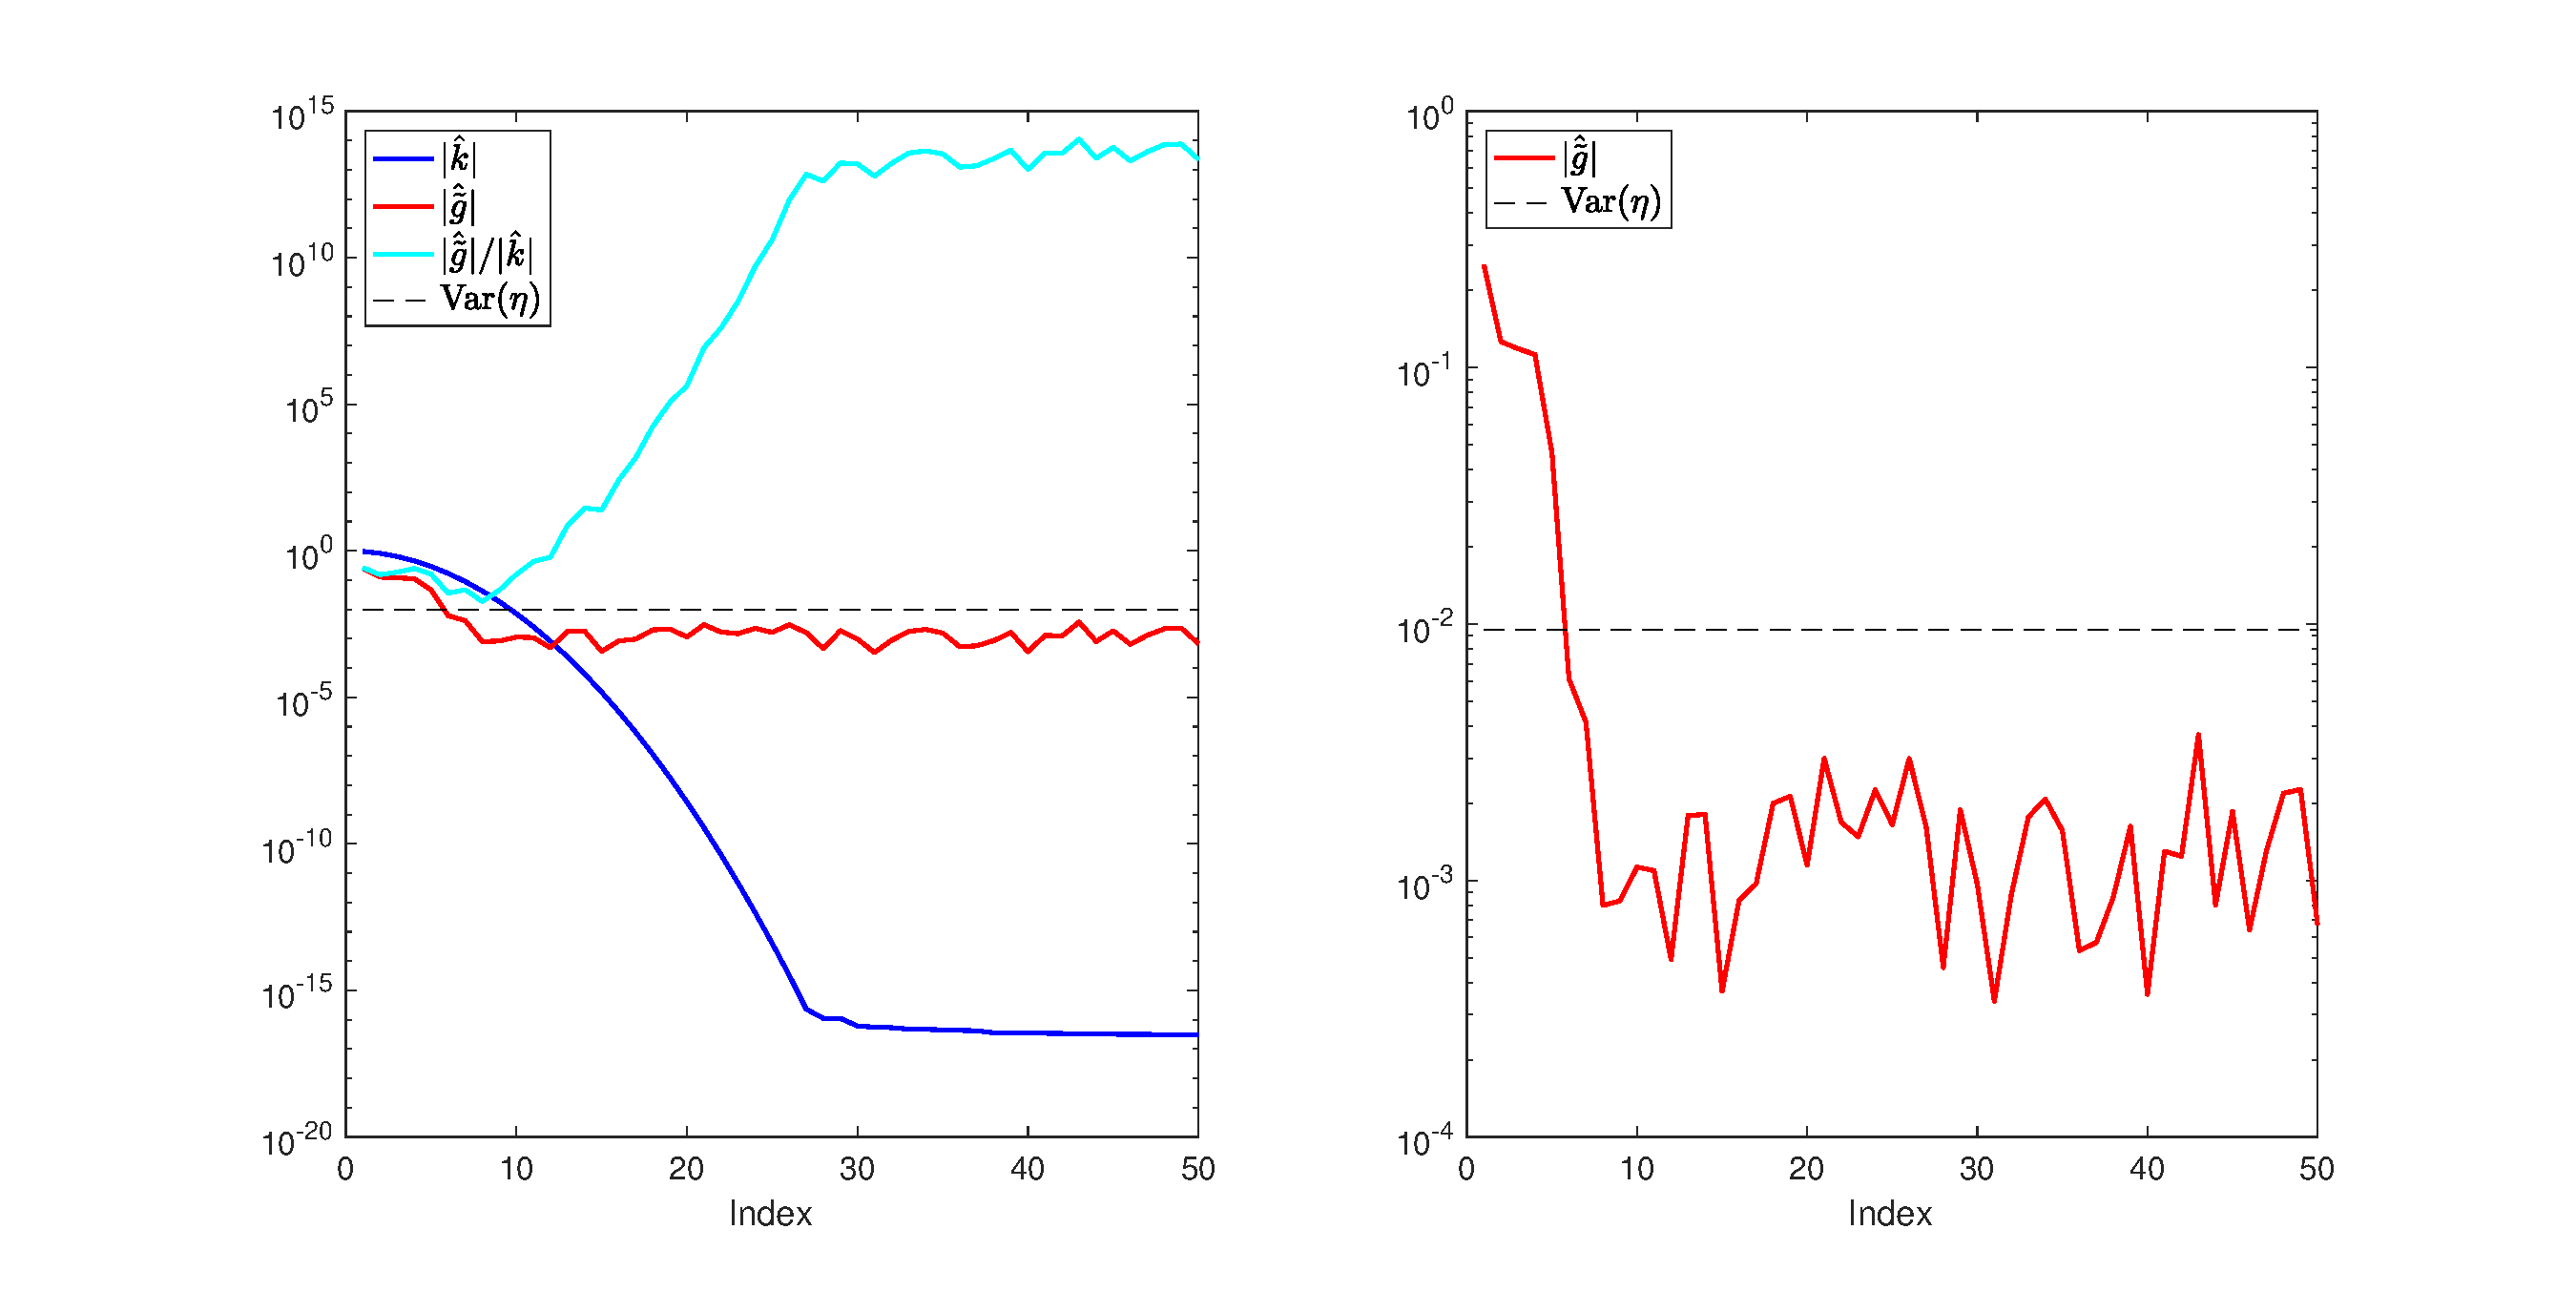
\includegraphics[scale = 0.45]{Figures/PicardPlot1D_F2_S15_W200.eps}}
\caption{(Left) A Picard plot generated from the second test function, a Gaussian blur with a width of 200, and an SNR of 15. The terms $|\widehat{\gnoise}_i|/|\widehat{\kdis}_i|$ decrease until index 8, at which case the terms increase in magnitude. This is due to the fact that the $|\widehat{\kdis}_i|$ steadily decrease, while the $|\widehat{\gnoise}_i|$ level off just below the variance in the noise. (Right) A zoom-in of the Picard plot is provided, showing that elements of the DFT of $\gnoise$ decay only slightly below the variance of the noise in $\gnoise$.}
\label{PicardPlot}
\end{figure}

\section{Experiment design} \label{Experiment design}

For the numerical experiments, three test functions are considered. While these functions vary in the extent of smoothness, all three functions are selected to be 1-periodic and the interval selected is [0,1], though this interval can be mapped to any other interval using a linear transformation. In general, the transformation from $[a,b]$ to $[c,d]$ such that $a \mapsto c$ and $b \mapsto d$ has a point-slope representation
\[y - c = \left(\frac{d-c}{b-a}\right)(x - a)\]
where $y \in [c,d]$ is the image of $x \in [a,b]$. \par
The first test function is $\fcon(x) = \cos(4\pi{t})\sin(6\pi{t})$, which is infinitely differentiable on all of $\mathbb{R}$. The second test function \eqref{Eq_TF2} is piecewise-smooth. The third and final test function is
\begin{equation}
\fcon(x) = \cos(8\pi{t})\exp(\sin(10\pi{t})-1)
\label{Eq_TF3}
\end{equation}
which is also infinitely differentiable on $\mathbb{R}$; the third function was selected to be more interesting than the first test function. Graphs of all three test functions are found in Figure \ref{TestFunctions}.  \par

\begin{figure}
	\centerline{\includegraphics[scale = 0.45]{Figures/TestFunctions1D.eps}}
\caption{The three test functions considered in the numerical experiments. Note that the second test function is only piecewise-smooth, while the first and second functions are smooth. All three functions are 1-periodic.}
\label{TestFunctions}
\end{figure}

The interval $[0,1]$ is discretized as equispaced points $0, 1/N, 2/N, \ldots, (N-1)/N$ for $N = 4096$. In other words, the interval is discretized as the vector $\tdis = [t_1,t_2,\ldots,t_N]$ with $t_i = (i-1)/N$. The selected test function $\fcon$ is then sampled at these points so that the discrete version $\fdis = [\fcon_1,\fcon_2,\ldots,\fcon_N]$ has elements $\fcon_i = \fcon(t_i)$. For the discrete version of $\kcon(x,t)$ to be used in the convolution with $\fdis$, the periodic extension of $\kcon(x,t)$ is sampled in the same way that was used to construct $\fdis$. However, it is important to remember that unextended $\kcon(x,t)$ was assumed to be centered at the origin and compactly supported on the interval $[-1/2,1/2]$. As such, a plot of $\kdis$ will not resemble the traditional graph of a Gaussian bump but instead be a depiction of a trough between bumps in the periodic extension of $\kcon$; see Figure \ref{RegAndTroughGaussian}. In the experiments, the width of the Gaussian kernels are chosen to be 100 and 200.  \par

\begin{figure}
	\centerline{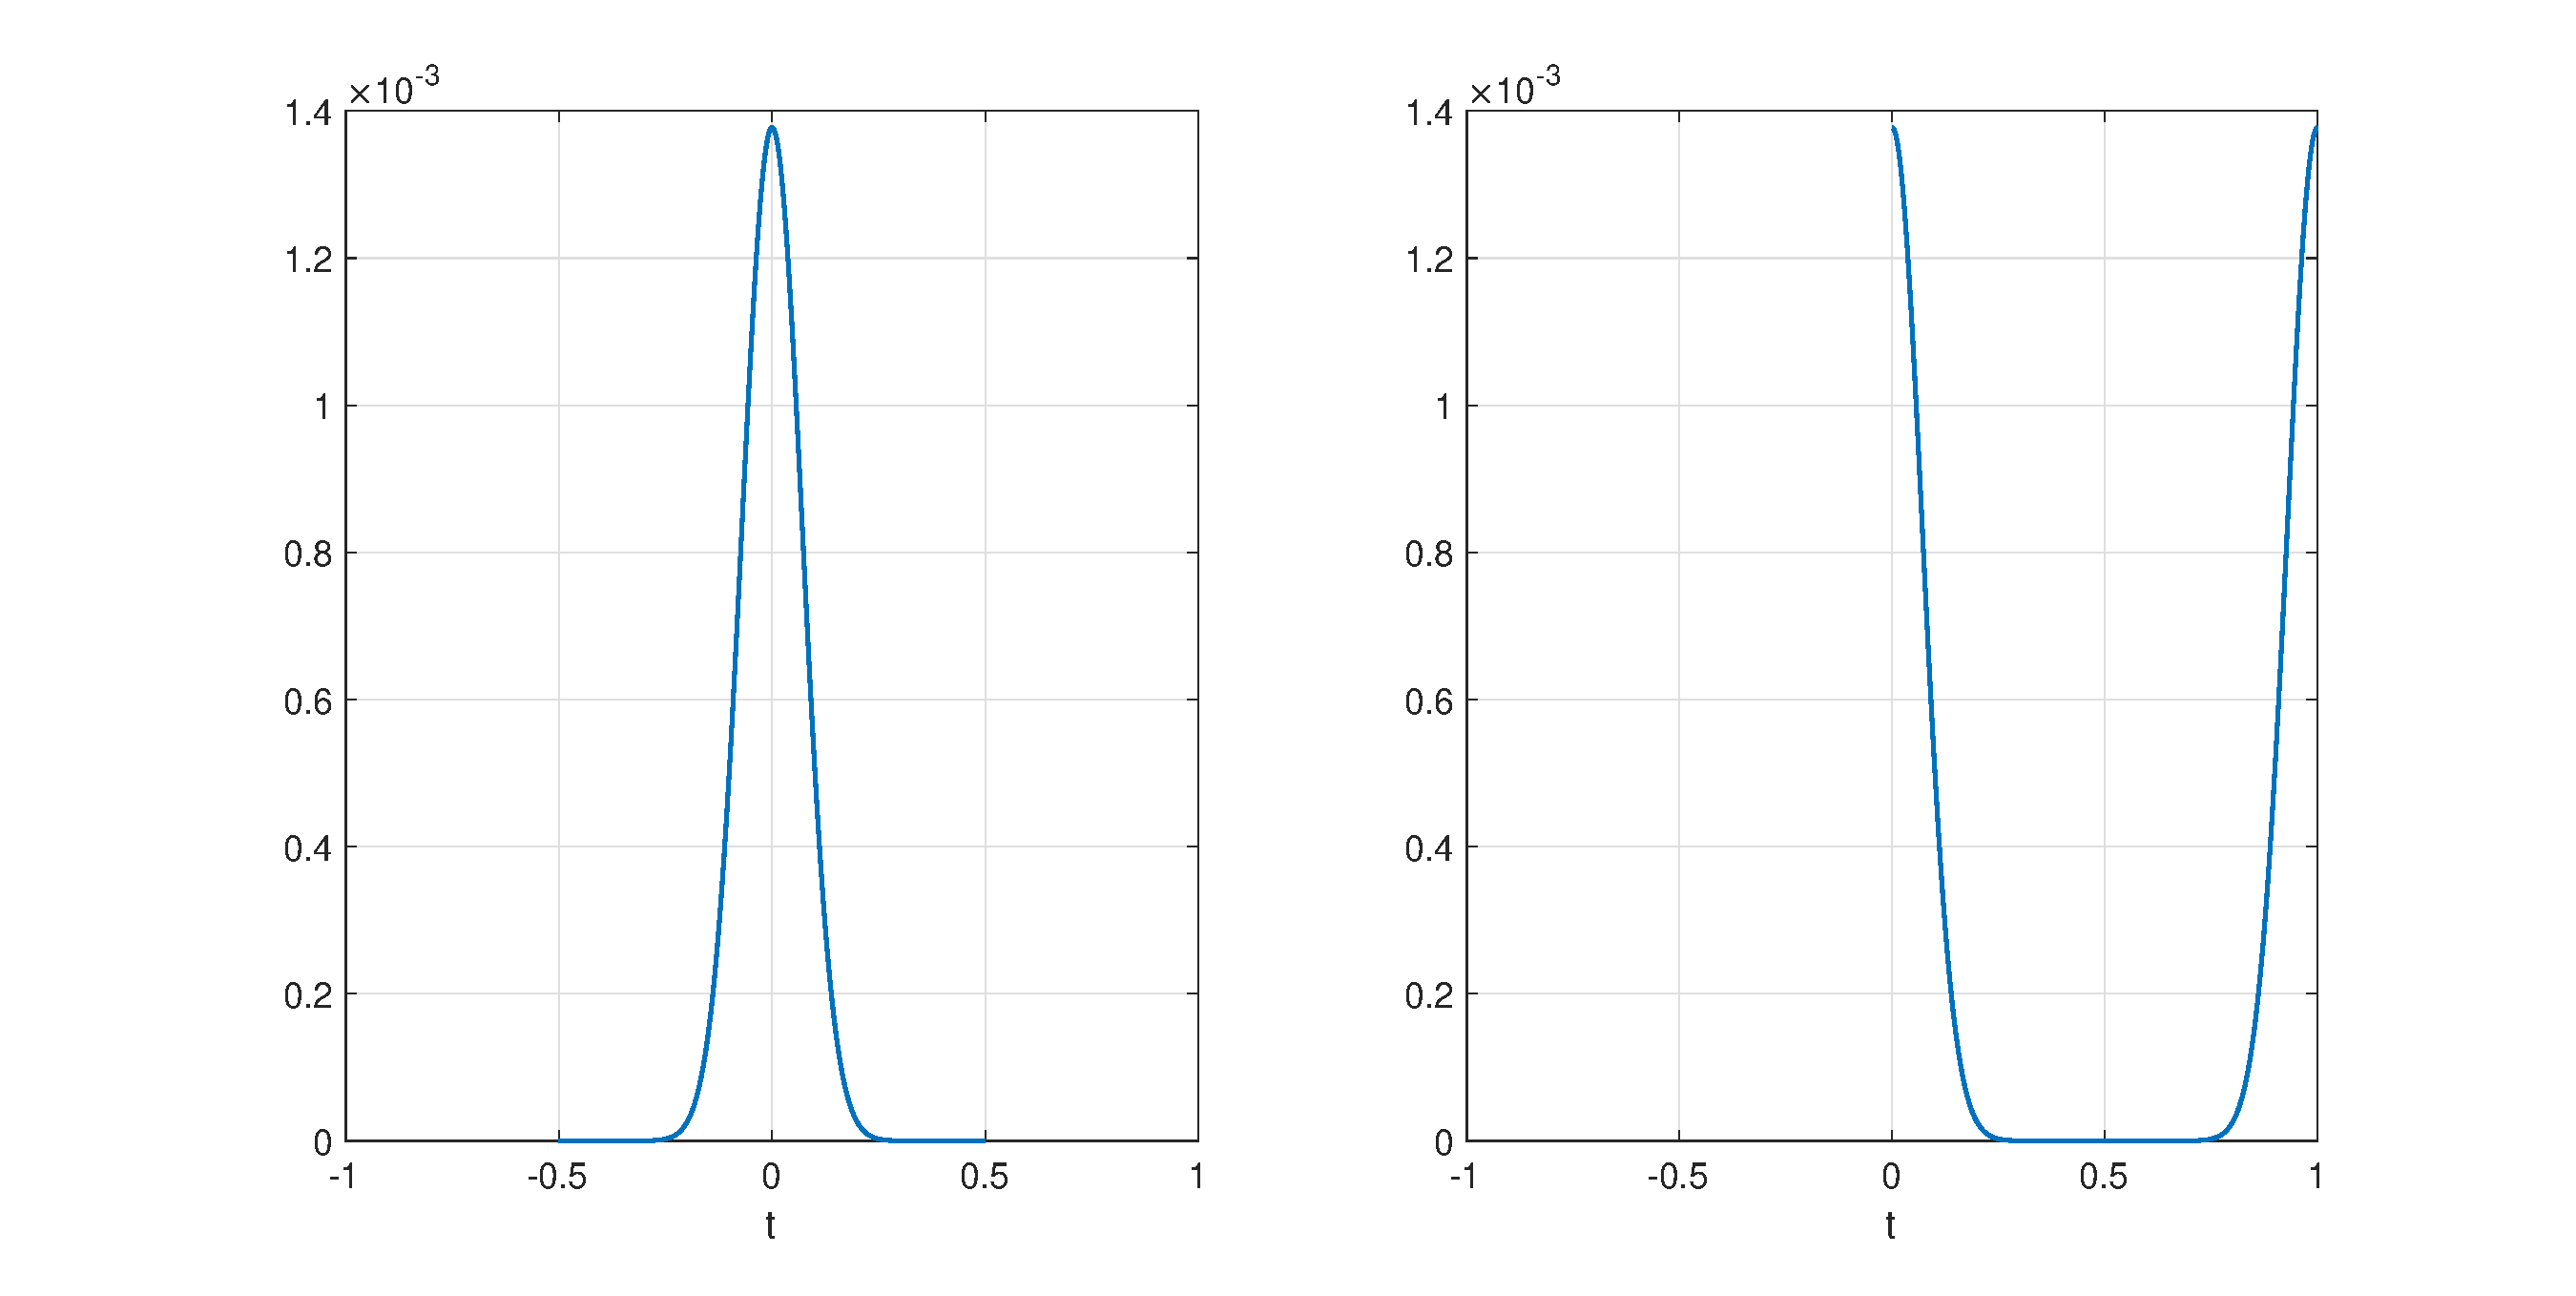
\includegraphics[scale = 0.45]{Figures/RegAndTroughGaussian.eps}}
\caption{Plots of different discretizations of the kernel $\kcon(t)$. The discretization on the left reflects the compact support of $\kcon(t)$ on the interval $[-1/2,1/2]$. The discretization on the right represents the periodic extension of $\kcon(t)$ on the interval $[0,1]$.}
\label{RegAndTroughGaussian}
\end{figure}

With the discretizations $\fdis$ and $\kdis$ determined, the discretization $\gdis$ of $\gcon(t)$ can be evaluation using either a circular convolution or a linear convolution with appropriate vector padding. Ultimately the vectors $\fdis$, $\kdis$, and $\gdis$ are vector discretizations of $\fcon(t)$, $\kcon(t)$, and $\gcon(t)$, respectively. \par
Overall, two selections for the width of the Gaussian kernel, two selections 5 and 25 for SNR value, and three test functions lead to a total of 12 experimental configurations. For each configuration, 20 noise realizations were generated and tested. The full resolution problem was constructed using $N = 4096$ points. The downsamped resolutions were selected as $n \in \{16,32,\ldots,2048\}$ for a total of nine resolutions (eight values of $n$).

\subsection{Construction of noise} \label{Construction of noise}

Though the definition of SNR varies, the definition chosen for this investigation is
\begin{equation}
\label{Eq_SNR}
\text{SNR} = 10\log_{10}\left(\frac{P_{\text{signal}}}{P_{\text{noise}}}\right)
\end{equation}
where $P$ denotes average power. In the discrete setting, the average power of a signal $\mathbf{f}$ of length $N$ is defined as $\|\mathbf{f}\|^2/N$. Using this definition, $P_{\text{signal}} = \|\gdis\|^2/N$ and $P_{\text{noise}} = \|\noise\|^2/N$ and so the quotient in the logarithm is $\|\gdis\|^2/\|\noise\|^2$. The quotient can also be expressed as $(\|\gdis\|/\|\gnoise - \gdis\|)^2$, which is the square of the multiplicative inverse of the relative error of $\gnoise$. \par
In MATLAB, the noise vector $\noise$ can be constructed by first taking an $N$-vector $\mathbf{e}$ drawn from the multivariate standard normal distribution and multiplying the vector by a constant $\noiseSD$. Doing so ensures that $\noise$ has variance $\noiseSD^2$ because $\Var(\noise) = \Var(\noiseSD\:\mathbf{e}) = \noiseSD^2\:\Var(\mathbf{e})$ and $\mathbf{e}$ has unit variance. Thus it is useful to rearrange the equation defining SNR into an equation that provides a way of finding the necessary variance for a given SNR value. The rearrangement is shown below, with $\|\noise\|^2$ replaced by $\E(\|\noise\|^2)$.
\[\E(\|\noise\|^2) = \frac{\|\gdis\|^2}{10^{(\text{SNR}/10)}}\]
Using the properties of expected value and the fact that $\E(\|\noise\|^2) = \E(\|\noiseSD\:\mathbf{e}\|^2)$, the term on the left hand side of the equation can be changed as
\[\E(\|\noise\|^2) = \E(\|\noiseSD\:\mathbf{e}\|^2) = \noiseSD^2 \sum_{i=1}^N \E(\mathbf{e}_i^2) = \noiseSD^2 \sum_{i=1}^N \left(\E(\mathbf{e}_i)^2 + \Var(\mathbf{e}_i)\right) = \noiseSD^2 \sum_{i=1}^N \left(0^2 + 1\right) = \noiseSD^2\:N.\]
Utilizing this change, the following equation for variance is obtained.
\begin{equation}
\label{Eq_Var}
\noiseSD^2 = \frac{\|\gdis\|^2}{N \cdot 10^{(\text{SNR}/10)}}
\end{equation}
This equation is used for the numerical construction of the noise vectors. SNR values of 5 and 25 are used to generate the white noise added to $\gdis$, and one such data realization is shown in Figure \ref{NoisePlot1D_F2_S05_W200}. \par

\begin{figure}
	\centerline{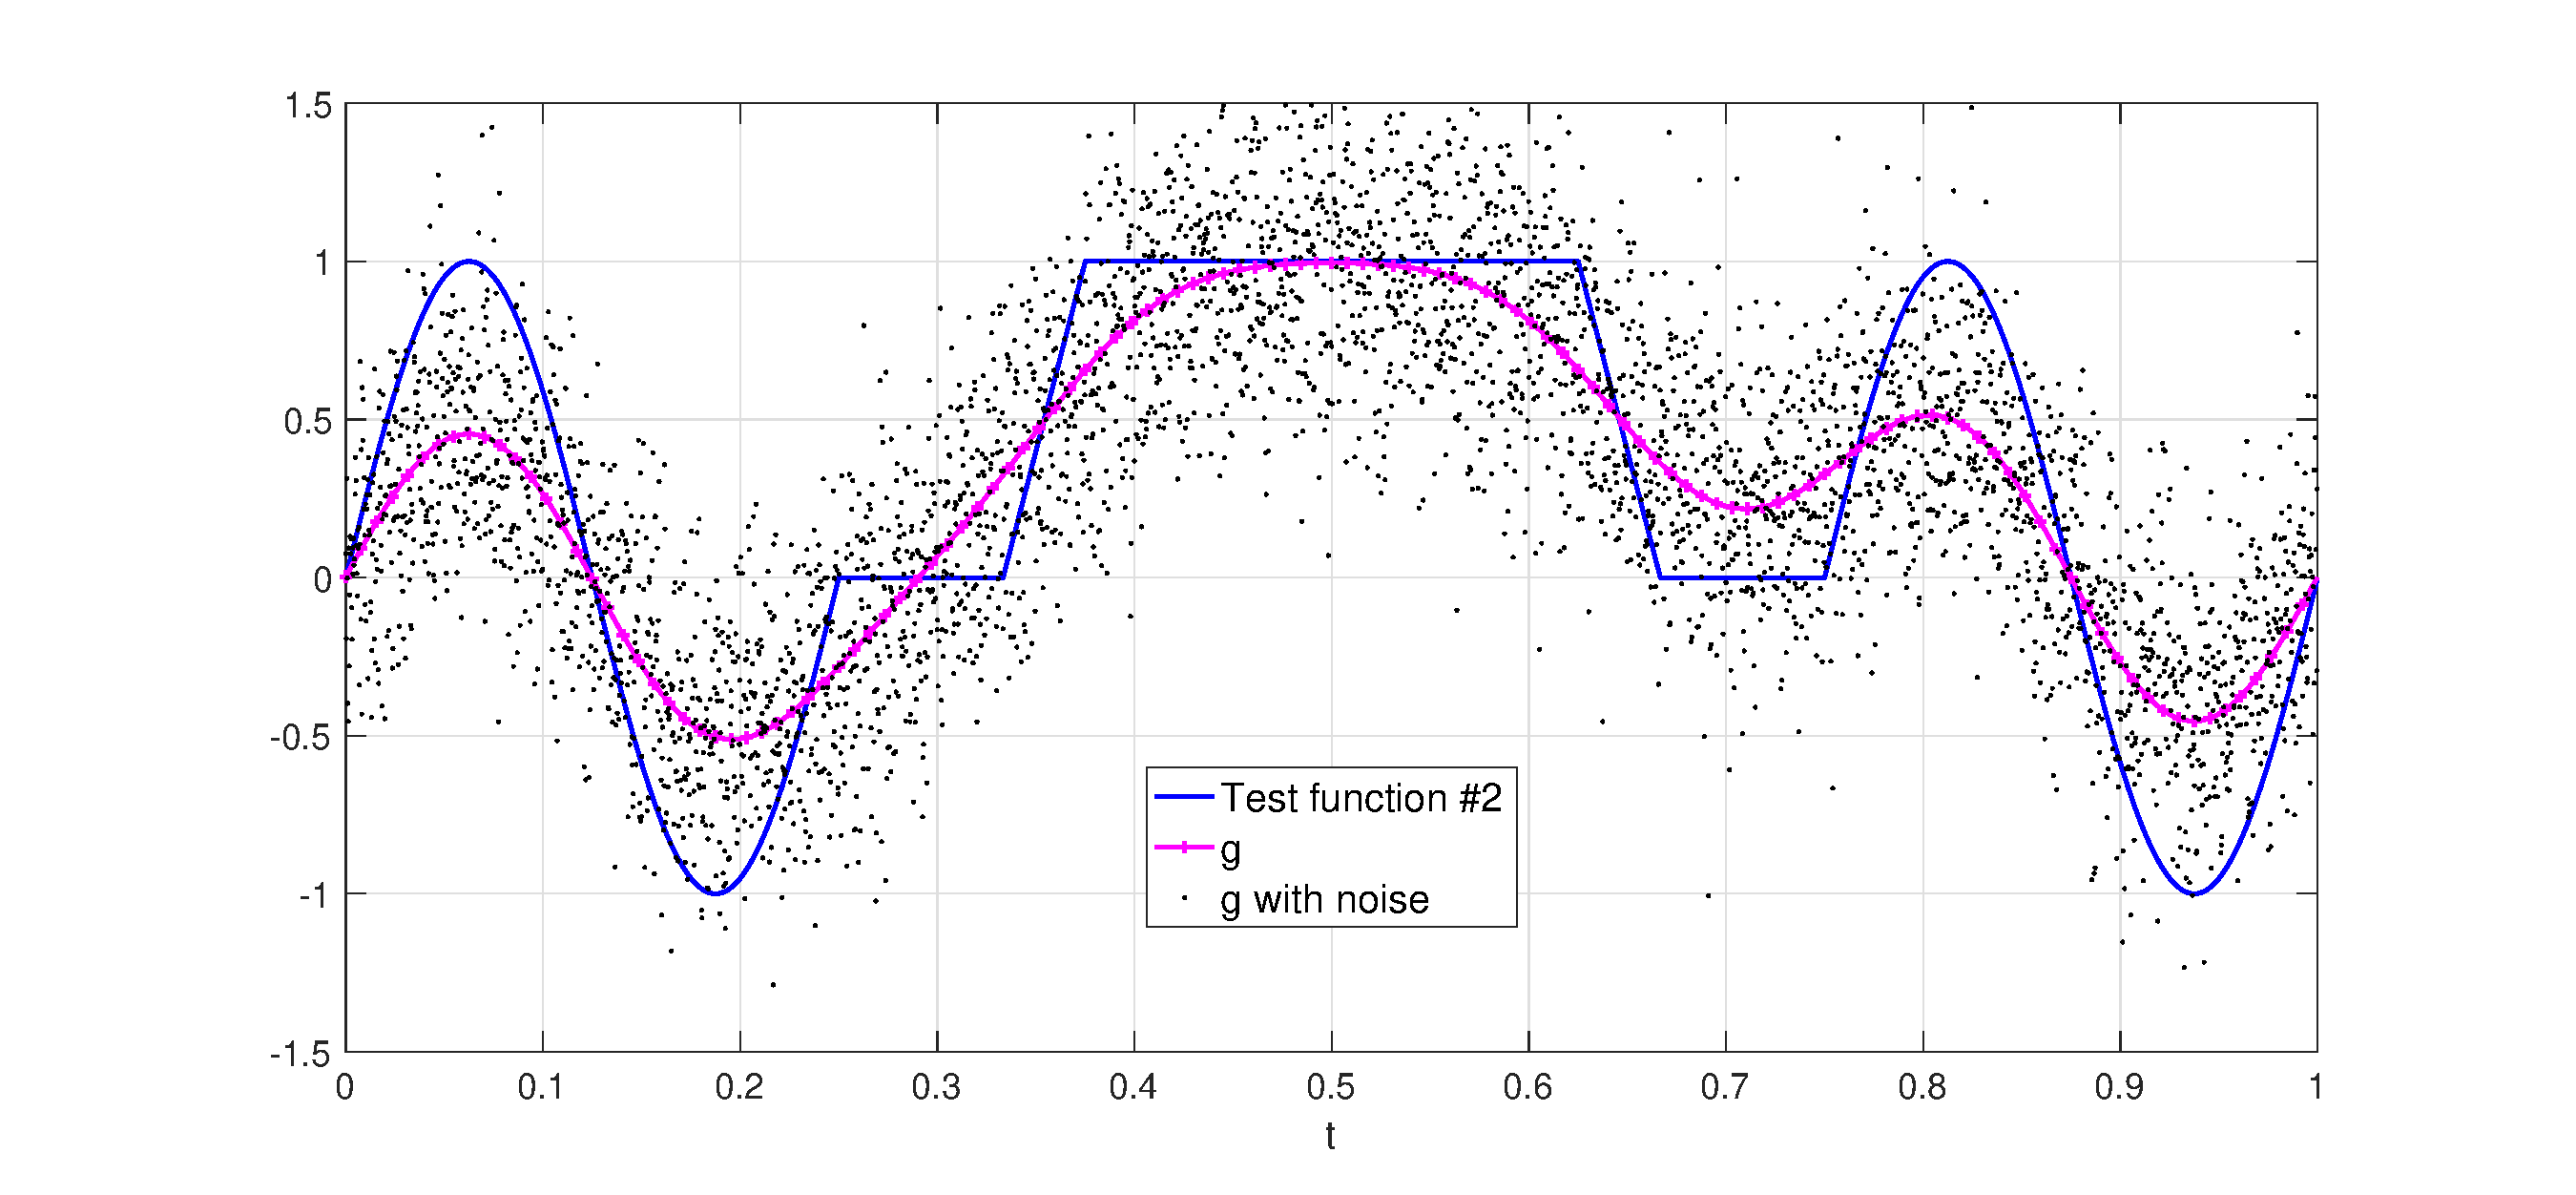
\includegraphics[scale = 0.45]{Figures/NoisePlot1D_F2_S05_W200.eps}}
\caption{The plot shows one data realization of $\gdis$ with noise, where the original function $f$ was the second test function. The SNR value is 5 and the width of the Gaussian PSF is 200.}
\label{NoisePlot1D_F2_S05_W200}
\end{figure}

For an accurate evaluation of the numerical experiments and their results, multiple realizations of noise are used. A primary advantage of multiple noise realizations is that the sample variance of noise vectors approaches the desired variance as the number of realizations increases. More rigorously, the mean of the sample variances of the noise vectors converges almost surely to the expected value of the sample variance, which is the desired variance $\noiseSD^2$; this is a direct consequence of the (strong) law of large numbers and the fact that the noise vectors are independent and identically distributed with standard normal distribution.  \par

%\begin{figure}
%\centerline{\includegraphics[scale=0.45]{Figures/LLN_Plot.eps}}
%\caption{The three plots correspond to the noise vectors generated using each of the three test functions (the right hand side of equation \eqref{Eq_Var} depends upon $\gdis$, which depends upon the test function $\fdis$ and the width of the Gaussian kernel). Equation \eqref{Eq_Var} also depends upon SNR; a SNR of 5 and Gaussian kernel width of 50 was used in all three cases. The horizontal axis represents the number of noise realizations and the vertical axis represents sample variance. All three plots show that as the number of realizations increases, the mean of the sample variances approaches the desired sample variance (the left hand side of equation \eqref{Eq_Var} and the red line in the plots).}
%\label{LLN_Plot}
%\end{figure}

Another numerical consideration regarding noise is how the sample variance changes across downsampling resolutions. To formalize the concept of downsampling in the context of this report, consider $\mathbf{z} = [z_1,z_2,\ldots,z_n]$. Then a vector $\mathbf{y}$ is called a downsampling of $\mathbf{z}$ if $\mathbf{y} = [z_{n_1},z_{n_2},\ldots,z_{n_m}]$, where $m \leq n$ and $n_j:\{1,2,\ldots,m\}\rightarrow\{1,2,\ldots,n\}$ is a strictly increasing function. This definition is analogous to the definition of a subsequence except with a finite number of terms. \par
Theoretically, the variance of the noise vector does not change when a vector is downsampled because of the properties of variance. For any $m\times n$ matrix $M$ and $n$-vector $\noise \sim \mathcal{N}(\bm{0},\noiseSD^2I)$
\begin{equation}
\Var(M\noise) = M\Var(\noise)M^{\trans} = \noiseSD^2MIM^{\trans} = \noiseSD^2MM^{\trans}
\label{Eq_VarProp}
\end{equation}
where $MM^\trans$ is an $m \times m$ matrix. Certainly for arbitrary $M$, $MM^\trans$ can differ from an $m \times m$ identity matrix, which would mean that the new noise vector $M\noise$ no longer represents white noise. However, given an $n$-vector $\noise \sim \mathcal{N}(\bm{0},\noiseSD^2I)$ and the goal of obtaining a downsampled version of $\noise$, a matrix $E$ can be found such that $E\noise$ is the downsampled vector. Since DFT's are utilized in the regularization process, a downsampled vector whose components are still equidistant from adjacent components is desirable. Since the finest sampling $\tdis$ of the interval $[0,1]$ has $N = 4096 = 2^{12}$ points, a natural downsampling with this property would be to select every other component of $\tdis$. The resulting downsampled vector would then have length $N/2 = 2048 = 2^{11}$. The matrix $E$ that accomplishes this downsampling is the $N/2 \times N$ matrix defined as
\begin{equation}
E = [\mathbf{e}_1 \: \mathbf{0} \: \mathbf{e}_2 \: \mathbf{0} \: \mathbf{e}_3 \: \mathbf{0} \ldots \mathbf{e}_N]
\label{Eq_E}
\end{equation}
where $\mathbf{0}$ is the $N/2$-vector of all zeros and $\mathbf{e}_j$ is the $N/2$-vector of all zeros except for 1 as the $j\text{th}$ component, $1 \leq j \leq N/2$. Another explanation of how to construct $E$ is to concatenate every other row of an $N \times N$ identity matrix. In an effort to clarify this downsampling process, let $\tdis^{n}$ denote the $n$-point downsampling of $\tdis$. Then with this new notation, $\tdis^{2046} = E\tdis$. \par
As a smaller example, consider the vector
\[\tdis = \begin{bmatrix}
0 & \dfrac{1}{8} & \dfrac{1}{4} & \dfrac{3}{8} & \dfrac{1}{2} & \dfrac{5}{8} & \dfrac{3}{4} & \dfrac{7}{8}
\end{bmatrix}^{\trans},\]
which is an equispaced 8-point discretization of $[0,1]$. The $4 \times 8$ matrix $E$ used to obtain downsampling $\tdis^{4}$ is
\[E = \begin{bmatrix}
1 & 0 & 0 & 0 & 0 & 0 & 0 & 0 \\
0 & 0 & 1 & 0 & 0 & 0 & 0 & 0 \\
0 & 0 & 0 & 0 & 1 & 0 & 0 & 0 \\
0 & 0 & 0 & 0 & 0 & 0 & 1 & 0 \\
\end{bmatrix}.\]
Then $\tdis^4$ obtained by the product $E\tdis$ has equispaced components as desired:
\[\tdis^4 = E\tdis = \begin{bmatrix}
0 & \dfrac{1}{4} & \dfrac{1}{2} & \dfrac{3}{4}
\end{bmatrix}^{\trans}.\]
\indent Another property of the $N/2 \times N$ matrix $E$ defined in \eqref{Eq_E} is that $EE^{\trans} = I$, where $I$ is the $N/2 \times N/2$ identity matrix.  This is a direct consequence of $\mathbf{e}_j\mathbf{e}_j^\trans = 1$ for all $j$ with $1 \leq j \leq N/2$. Using the property in \eqref{Eq_VarProp}, the variance of the  noise vector $\noise^{N/2}$ downsampled from $\noise$ is then
\[\Var(\noise^{N/2}) = \Var(E\noise) = E\Var(\noise)E^{\trans} = \noiseSD^2EE^{\trans} = \noiseSD^2I\]
where $I$ is the $N/2 \times N/2$ identity matrix. Therefore, downsampling white noise vectors in this way produces white noise vectors of half length, theoretically preserving variance across downsamples. As a final remark, the process of downsampling described here can be used to obtain downsampled vectors of length $N/(2^2), N/(2^3), \ldots, N/N$, though the final resolution in this report has been chosen as $N/(2^8) = 16$. \par 
While the variance of the noise is preserved across downsampling resolution in theory, numerically there is some fluctuation. As the downsampling resolutions decrease, i.e. the length of the downsampled vectors decreases, the sample variances more spread out. Figure \ref{VarPlot1D} demonstrates this phenomenon by showing boxplots of sample variance versus downsampling resolutions. 

\begin{figure}
\centerline{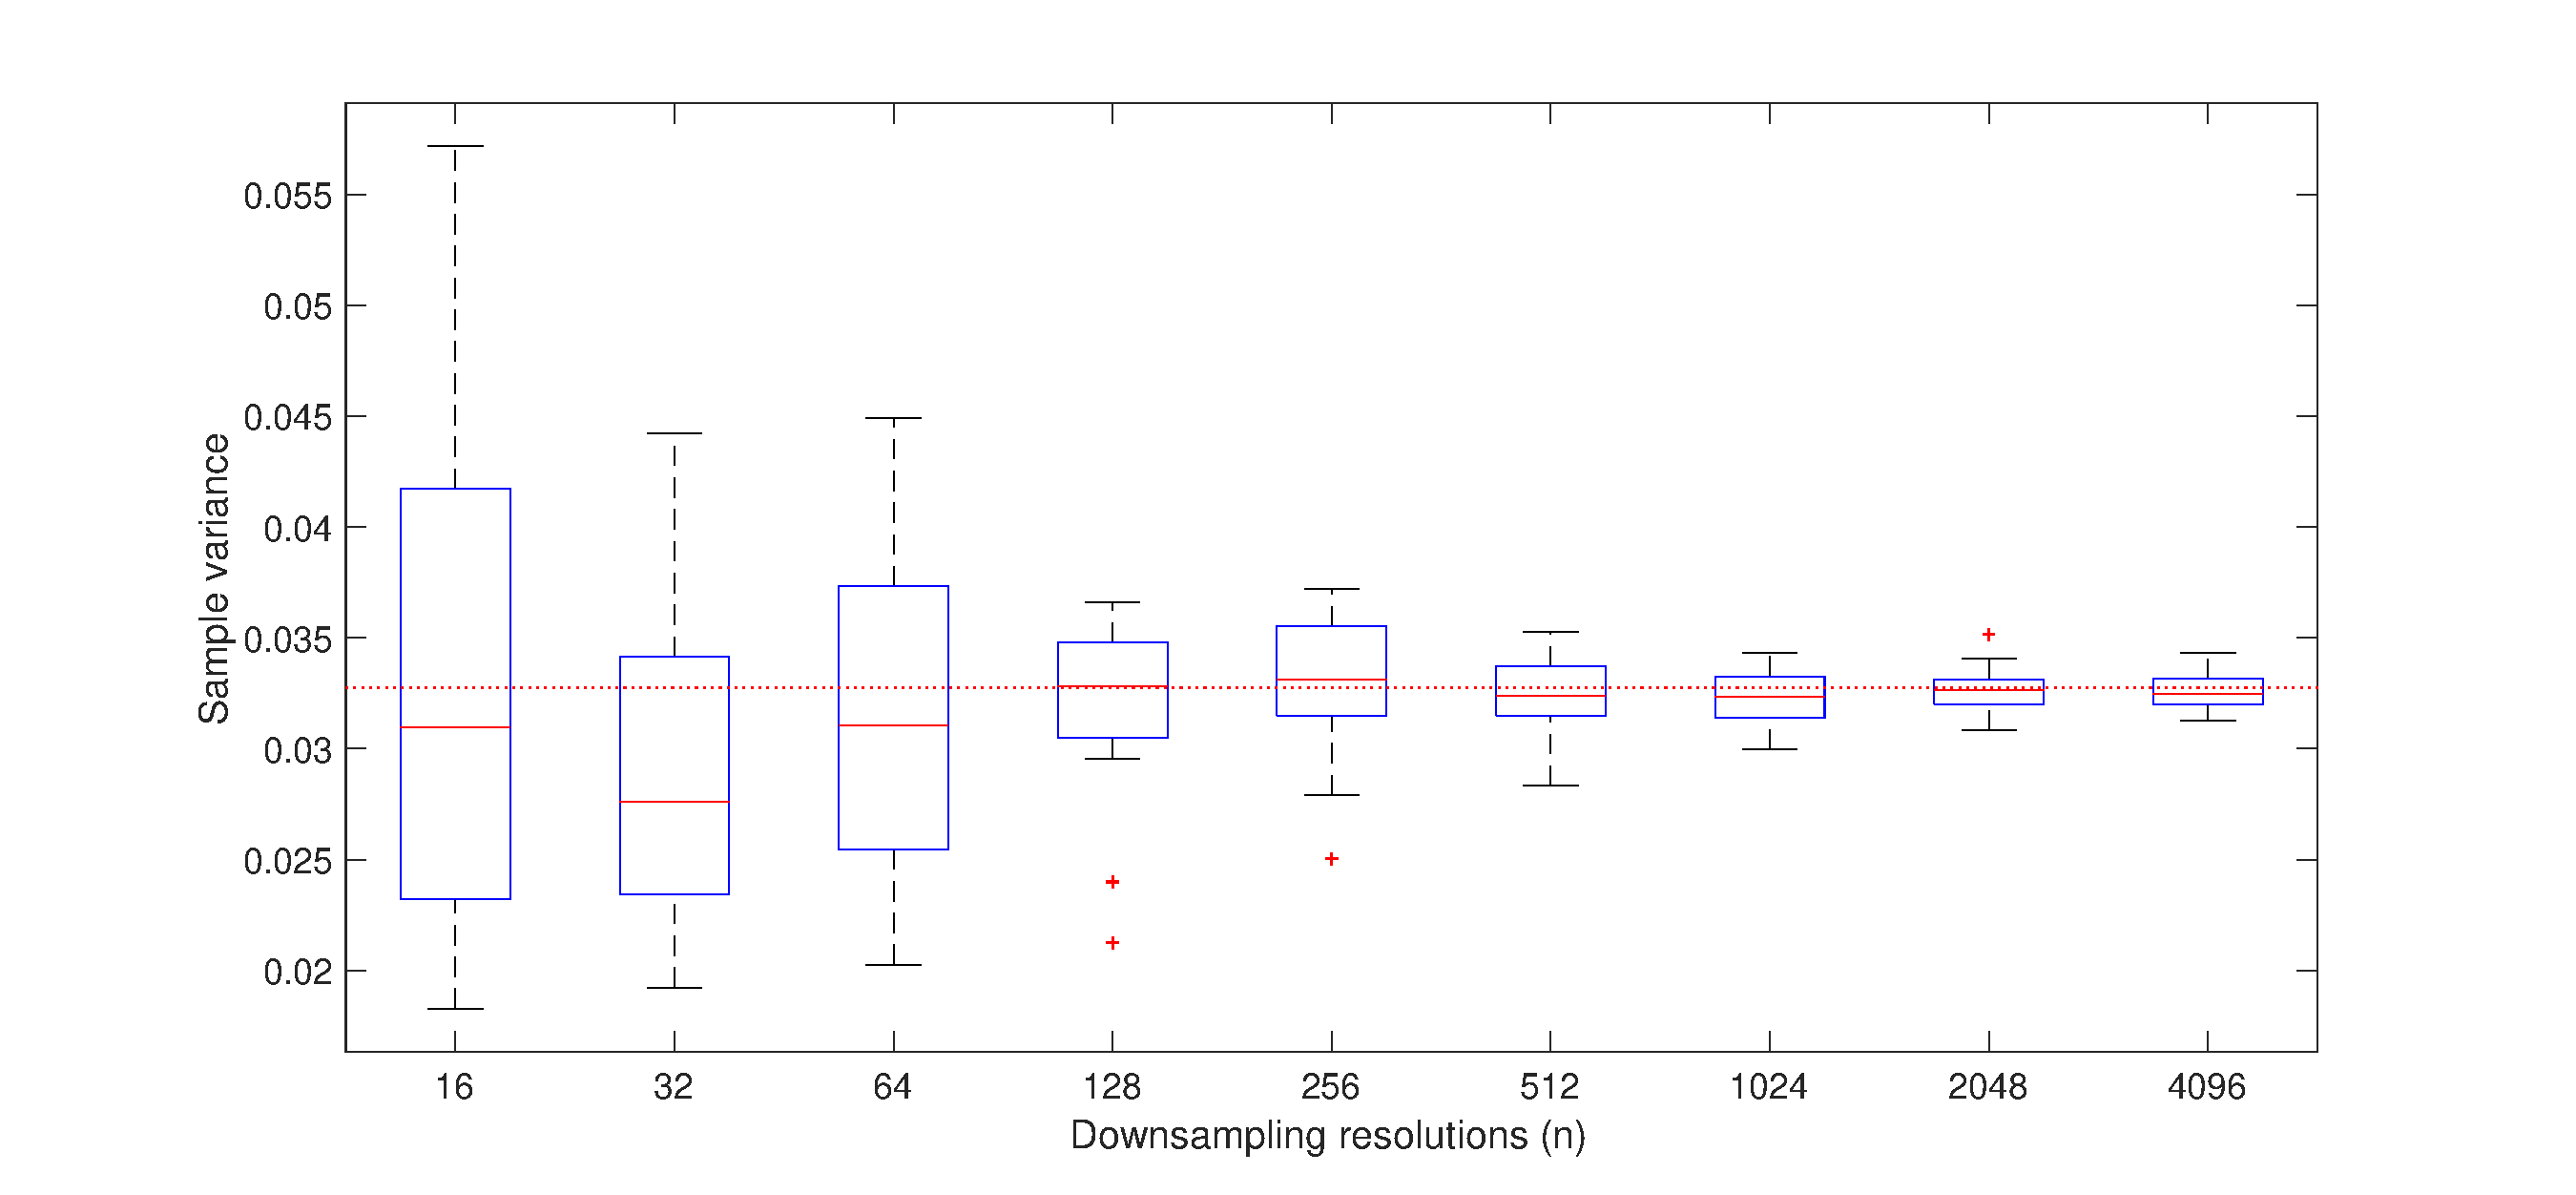
\includegraphics[scale=0.45]{Figures/VarPlot1D_F1_S05_W100_R20.eps}}
\caption{The boxplots were generated from the sample variances of downsampled noise vectors. The theoretical variance of the noise was set to 0.0327, which is indicated by the horizontal dotted line. This figure illustrates that as the lengths of the downsampled vectors decrease, the variance in the computed sample variances increases.}
\label{VarPlot1D}
\end{figure}

\section{Parameter estimation methods} \label{Parameter estimation methods}

\subsection{Unbiased Predictive Risk Estimator} \label{Unbiased Predictive Risk Estimator}
The Unbiased Predictive Risk Estimator (UPRE) method is derived by considering the following quantity
\[\PE := \kmat(\freg - \fdis)\]
This quantity $\PE$ is known as the \textit{predictive error}, and is an alternative to solution error defined as $\freg - \fdis$. Given the above definition, the mean squared norm of the predictive error is
\[\frac{1}{n}\|\PE\|^2 = \frac{1}{n}\|\kmat(\freg - \fdis)\|^2\]
which is called the predictive risk.  As a first step in deriving the UPRE method, assume that the noise $\noise$ is a random vector, instead of a realization of a random vector. Direct consequences of this assumption are that $\gdis$ and $\freg$ are random vectors and the predictive risk $(1/n)\|\PE\|^2$ is a random variable. \par
Next, an $n \times n$ matrix $\A$ is defined as $\A = \kmat\R$ where $\R$ is a regularization matrix. The notation $\A$ is chosen to indicate that the matrix depends upon the regularization parameter contained in $\R$. Using the influence matrix with $\freg = \R\gnoise$, the predictive error can be rewritten:
\begin{align*}
\PE &= \kmat\freg - \kmat\fdis \\
&= \A\gnoise - \kmat\fdis \\
&= \A(\kmat\fdis + \noise) - \kmat\fdis \\
&= (\A - I)\kmat\fdis + \A\noise
\end{align*}
By the assumption that $\noise$ is a discrete white noise vector, the Trace Lemma can be utilized to obtain an expression for the expected value of predictive risk.

\begin{TL}
Let $f \in \mathcal{H}$, where $\mathcal{H}$ is a deterministic, real Hilbert space, let $\noise$ be a discrete noise vector with $\noise \sim \mathcal{N}(0,\noiseSD^2)$, and let $B: \mathbb{R}^n \rightarrow \mathcal{H}$ be a bounded linear operator. Then
\[\E(\|f + B\noise\|_{\mathcal{H}}^2) = \|f\|_{\mathcal{H}}^2 + \noiseSD^2\trace({B^*}B)\]
where $B^*$ denotes the adjoint of $B$.
\end{TL}
\begin{proof}
By the linearity of inner products and the expected value operator,
\[\E(\|f + B\noise\|_{\mathcal{H}}^2) = \E(\langle f + B\noise, f + B\noise\rangle_{\mathcal{H}}) = \E(\|f\|_{\mathcal{H}}^2) + 2\E(\langle f, B\noise\rangle_{\mathcal{H}}) + \E(\langle B\noise, B\noise\rangle_{\mathcal{H}}).\]
The term $\E(\|f\|_{\mathcal{H}}^2)$ reduces to $\|f\|_{\mathcal{H}}^2$ because $f$ is an element of a deterministic Hilbert space. Next, the inner products can be rewritten using the adjoint of $B$:
\begin{align*}
\E(\|f + B\noise\|_{\mathcal{H}}^2) &= \|f\|_{\mathcal{H}}^2 + 2\E(\langle f, B\noise\rangle_{\mathcal{H}}) + \E(\langle B\noise, B\noise\rangle_{\mathcal{H}}) \\
&= \|f\|_{\mathcal{H}}^2 + 2\E(({B^*}f)^\trans\noise) + \E({\noise^\trans}{B^*}B\noise) \\
&= \|f\|_{\mathcal{H}}^2 + 2\sum_{i=1}^n ({B^*}f)_i \E(\noise_i) + \sum_{i=1}^n\sum_{j=1}^n ({B^*}B)_{ij} \E({\noise_i}{\noise_j})
\end{align*}
Since $\noise \sim \mathcal{N}(0,\noiseSD^2)$, the expected values of $\noise_i$ and ${\noise_i}{\noise_j}$ are zero and $\noiseSD^2\delta_{ij}$, respectively. Therefore the second term above is zero and the third term is a summation expression for $\noiseSD^2\trace({B^*}B)$.
\end{proof}

\noindent Applying the Trace Lemma to the expression for predictive risk yields
\[\E\left(\frac{1}{n}\|\PE\|^2\right) = \frac{1}{n}\E\left(\|(\A-I)\kmat\fdis + \A\noise\|^2\right) = \frac{1}{n}\|(\A-I)\kmat\fdis\|^2 + \frac{\noiseSD^2}{n}\trace({\A^\trans}\A).\]
If Tikhonov regularization is used, then the influence matrix $\A$ is $\kmat(\kmat^\ctrans\kmat + \regparam{D^\ctrans}D)^{-1}\kmat^\ctrans$. The matrix $(\kmat^\ctrans\kmat + \regparam{D^\ctrans}D)^{-1}$ is symmetric as a result of $\kmat^\ctrans\kmat$ and $\regparam{D^\ctrans}D$ being individually symmetric, and thus the corresponding influence matrix $\A$ is symmetric.  With a symmetric matrix $\A$, the expected value of predictive risk is simplified to
\begin{equation}
\label{Eq_PR}
\E\left(\frac{1}{n}\|\PE\|^2\right) = \frac{1}{n}\|(\A-I)\kmat\fdis\|^2 + \frac{\noiseSD^2}{n}\trace(\A^2).
\end{equation}
\indent The last step in the derivation of the UPRE method is to introduce the \textit{regularized residual}, which is defined as $\regres = \kmat\freg - \gnoise$. The regularized residual is important because it is also used in the derivation of the generalized cross validation and discrepancy principle methods. Using the influence matrix $\A$, the expression for $\regres$ can also be written as
\[\regres = (\A-I)\gnoise = (\A-I)(\kmat\fdis + \noise) = (\A-I)\kmat\fdis + (\A-I)\noise.\]
By the Trace Lemma and the expression for $\regres$, the expected value of $(1/n)\|\regres\|^2$ is
\[\E\left(\frac{1}{n}\|\regres\|^2\right) = \frac{1}{n}\|(\A-I)\kmat\fdis\|^2 + \frac{\noiseSD^2}{n}\trace({(\A-I)^\trans}(\A-I))\]
For symmetric $\A$, the term $(\A-I)^\trans(\A-I)$ becomes $(\A-I)^2 = \A^2 - 2\A + I$ and so by the linearity of the trace operator,
\begin{equation}
\label{Eq_RR}
\E\left(\frac{1}{n}\|\regres\|^2\right) = \frac{1}{n}\|(\A-I)\kmat\fdis\|^2 + \frac{\noiseSD^2}{n}\trace(\A^2) - \frac{2\noiseSD^2}{n}\trace(\A) + \noiseSD^2.
\end{equation}
By comparing \eqref{Eq_PR} and \eqref{Eq_RR}, the equation for the expected value of $(1/n)\|\PE\|^2$ can be expressed as
\[\E\left(\frac{1}{n}\|\PE\|^2\right) = \E\left(\frac{1}{n}\|\regres\|^2\right) + \frac{2\noiseSD^2}{n}\trace(\A) - \noiseSD^2.\]
The UPRE is defined to be
\begin{equation}
\label{Eq_UPRE}
\U(\regparam) = \frac{1}{n}\|\regres\|^2 + \frac{2\noiseSD^2}{n}\trace(\A) - \noiseSD^2
\end{equation}
and the UPRE method is to pick $\regparam_{\text{UPRE}} = \argmin \U(\regparam)$. \par 
Since the DFT is a the primary tool in the experiment, a spectral form of the UPRE function (one that involves DFT's) is desirable, as are spectral forms of the GCV and discrepancy principal functions in Sections \ref{Generalized Cross Validation} and \ref{Discrepancy Principle}. To derive a spectral form of \eqref{Eq_UPRE}, first recall that for Tikhonov regularization, $\A = \kmat(\kmat^\ctrans\kmat + \regparam{D^\ctrans}D)^{-1}\kmat^\ctrans$. From \eqref{Eq_CircDiag}, $\kmat = F^*\Delta{F}$, where $\Delta = \diag(\widehat{\kdis})$. If $D = F^\ctrans\Lambda{F}$ as well (with $\Lambda = \diag(\widehat{\ddis})$), then
\begin{align*}
\A &= \kmat(\kmat^\ctrans\kmat + \regparam{D^\ctrans}D)^{-1}\kmat^\ctrans \\
&= F^*\Delta{F}((F^*\Delta{F})^\ctrans F^\ctrans\Delta{F} + \regparam(F^\ctrans\Lambda{F})^\ctrans F^\ctrans\Lambda{F})^{-1}(F^*\Delta{F})^\ctrans \\
&= F^\ctrans\Delta{F}(F^\ctrans\Delta^\ctrans\Delta{F} + \regparam{F^\ctrans\Lambda^\ctrans\Lambda{F}})^{-1}F^\ctrans\Delta^\ctrans{F} \\
&= F^\ctrans\Delta{F}(F^\ctrans(\Delta^\ctrans\Delta + \regparam\Lambda^\ctrans\Lambda)F)^{-1}F^\ctrans\Delta^\ctrans{F} \\
&= F^\ctrans\Delta{F}F^\ctrans(\Delta^\ctrans\Delta + \regparam\Lambda^\ctrans\Lambda)^{-1}FF^\ctrans\Delta^\ctrans{F} \\
&= F^\ctrans\Delta(\Delta^\ctrans\Delta + \regparam\Lambda^\ctrans\Lambda)^{-1}\Delta^\ctrans{F}.
\end{align*}
The matrix $\Delta(\Delta^\ctrans\Delta + \regparam\Lambda^\ctrans\Lambda)^{-1}\Delta^\ctrans$ is diagonal, and so its diagonal entries are the the eigenvalues of $\A$. Then by definition of $\Delta$ and $\Lambda$, the $i$th diagonal entry of $\Delta(\Delta^\ctrans\Delta + \regparam\Lambda^\ctrans\Lambda)^{-1}\Delta^\ctrans$ is $|\widehat{\kdis}_i|^2/(|\widehat{\kdis}_i|^2 + \regparam|\widehat{\ddis}_i|^2)$. Therefore,
\begin{equation}
\trace(\A) = \sum_{i = -n/2}^{(n/2)-1} \frac{|\widehat{\kdis}_i|^2}{|\widehat{\kdis}_i|^2 + \regparam|\widehat{\ddis}_i|^2} = \sum_{i = -n/2}^{(n/2)-1} \filt(\regparam,|\widehat{\kdis}_i|)
\label{Eq_TraceUPRE}
\end{equation}
where $\filt$ is the Tikhonov filter function \eqref{Eq_TikFilt}. Since the operator $D$ is fixed, $\widehat{\ddis}$ can be pre-computed; this is reflected by the notation $\filt(\regparam,|\widehat{\kdis}_i|)$. \par
Next, the definition of $\regres$ gives
\[\frac{1}{n}\|\regres\|^2 = \frac{1}{n}\|\kmat\freg - \gnoise\|^2 = \sum_{i = -n/2}^{(n/2)-1} |\widehat{\kdis}_i\widehat{(\freg)}_i - \widehat{\gnoise}_i|^2.\]
and \eqref{Eq_TikSol} then produces
\begin{equation}
\frac{1}{n}\|\regres\|^2 = \sum_{i = -n/2}^{(n/2)-1} |\filt(\regparam,|\widehat{\kdis}_i|)\widehat{\gnoise}_i - \widehat{\gnoise}_i|^2 = \sum_{i = -n/2}^{(n/2)-1} |\widehat{\gnoise}_i|^2(1 - \filt(\regparam,|\widehat{\kdis}_i|))^2.
\label{Eq_RegResNorm}
\end{equation}
Combining \eqref{Eq_TraceUPRE} and \eqref{Eq_RegResNorm} produces the spectral from of the UPRE function:
\begin{equation}
\U(\regparam) = \sum_{i = -n/2}^{(n/2)-1} |\widehat{\gnoise}_i|^2(1 - \filt(\regparam,|\widehat{\kdis}_i|))^2 + \frac{2\noiseSD^2}{n}\sum_{i = -n/2}^{(n/2)-1} \filt(\regparam,|\widehat{\kdis}_i|) - \noiseSD^2.
\label{Eq_SpectralUPRE}
\end{equation} 
Since the UPRE method relies on finding a minimum of \eqref{Eq_SpectralUPRE}, the constant $\noiseSD^2$ can be ignored during implementation. In an effort to be more descriptive (note that \eqref{Eq_SpectralUPRE} also relies upon $n$), define
\begin{equation}
\U_n(\regparam) = \sum_{i = -n/2}^{(n/2)-1} |\widehat{\gnoise}_i|^2(1 - \filt(\regparam,|\widehat{\kdis}_i|))^2 + \frac{2\noiseSD^2}{n}\sum_{i = -n/2}^{(n/2)-1} \filt(\regparam,|\widehat{\kdis}_i|).
\label{Eq_SpectralUPREn}
\end{equation} \par 
Now consider the case where multiple data sets are available, which can arise from repeated observations of some time-invariant event. As an alternative to finding a regularization parameter for each data set, a single regularization parameter can be obtained by constructing a summed version of \eqref{Eq_SpectralUPREn}, assuming that $n$ is constant across all data sets to be considered. It is reasonable to expect that this single regularization parameter will perform worse that each individual parameter with respect to their corresponding data sets. However, computational time/resources could be saved because the method would involved solving a single minimization problem instead of solving a minimization problem for each data set. To bring this idea to fruition, some notation will be expanded. Let $R$ be the number of available data sets, and denote the $j$th data set by $\gnoise^j$. Similarly, let $\U_n^j(\regparam)$ be the UPRE function associated with the $j$th data set.  The sum of the UPRE functions is then 
\begin{align*}
\sum_{j=1}^R \U_n^j(\regparam) &= \sum_{j=1}^R \left(\sum_{i = -n/2}^{(n/2)-1} |\widehat{\gnoise^j}_i|^2(1 - \filt(\regparam,|\widehat{\kdis}_i|))^2 + \frac{2\noiseSD^2}{n}\sum_{i = -n/2}^{(n/2)-1} \filt(\regparam,|\widehat{\kdis}_i|)\right) \\
&= \sum_{j=1}^R \left(\sum_{i = -n/2}^{(n/2)-1} |\widehat{\gnoise^j}_i|^2(1 - \filt(\regparam,|\widehat{\kdis}_i|))^2\right) + \sum_{j=1}^R \left(\frac{2\noiseSD^2}{n}\sum_{i = -n/2}^{(n/2)-1} \filt(\regparam,|\widehat{\kdis}_i|)\right).
\end{align*}
By factoring terms from the first sum and noting that the summand of the second sum does not depend upon $j$, the function simplifies to
\begin{equation}
\sum_{j=1}^R \U_n^j(\regparam) =  \sum_{i = -n/2}^{(n/2)-1} \left(\sum_{j=1}^R |\widehat{\gnoise^j}_i|^2\right)(1 - \filt(\regparam,|\widehat{\kdis}_i|))^2 +  R\frac{2\noiseSD^2}{n}\sum_{i = -n/2}^{(n/2)-1} \filt(\regparam,|\widehat{\kdis}_i|).
\label{Eq_SpectralUPREsum}
\end{equation}
Numerically, \eqref{Eq_SpectralUPREsum} can be readily obtained by summing the DFT's of the data sets; note that $\widehat{\kdis}$ is unchanged across data sets. \par
To emphasize the validity of considering $\sum_{j=1}^R \U_n^j(\regparam)$, consider the following justification. If $F^j(x)$ are a collection of differentiable functions for $j = 1,\ldots,R$ (again $j$ represents the index of the function rather than the number of compositions or derivatives) with the same local minimizer $x_0$, then from calculus,
\[\frac{d}{dx}\left(\sum_{j=1}^R F^j(x)\right) = \sum_{j=1}^R \frac{dF^j}{dx}(x) \quad \text{and} \quad \sum_{j=1}^R \frac{dF^j}{dx}(x_0) = \sum_{j=1}^R 0 = 0.\]
Thus $x_0$ is also a minimizer of the sum of the $F^j(x)$. Even when the $F^j(x)$ do not have the same minimizer, if the minimizers $x_0^j$ of $F^j(x)$ (respectively) are contained within an interval $[a,b]$, then $\sum_{j=1}^R F^j(x)$ has a local minimum contained in $[a,b]$ (this seems to be the case but I don't have a proof yet).

\subsection{Generalized Cross Validation} \label{Generalized Cross Validation}
The UPRE method requires knowledge of the variance $\noiseSD^2$ of the noise vector $\noise$. In contrast, the generalized cross validation (GCV) method does not require knowledge of $\noiseSD^2$. The GCV functional is
\begin{equation}
\label{Eq_GCV}
\GCV(\regparam) = \frac{\frac{1}{n}\|\regres\|^2}{\left[\frac{1}{n}\trace(I-\A)\right]^2},
\end{equation}
where $\regres$ is the regularized residual defined in the derivation of the UPRE method. Similarities between the GCV and UPRE methods are that both functionals are estimators of the predictive risk, and the regularization parameter $\regparam$ is chosen as the minimizers of these functionals. \par 
By the linearity of the trace operator, $\trace(I-\A) = \trace(I)-\trace(\A) = n - \trace(\A)$. Then by \eqref{Eq_TraceUPRE},
\begin{equation}
\trace(I-\A) = n - \sum_{i = -n/2}^{(n/2)-1} \filt(\regparam,|\widehat{\kdis}_i|) = \sum_{i = -n/2}^{(n/2)-1} 1 - \filt(\regparam,|\widehat{\kdis}_i|).
\label{Eq_TraceGCV}
\end{equation}
Substituting \eqref{Eq_RegResNorm} and \eqref{Eq_TraceGCV} into \eqref{Eq_GCV} produces the spectral form of the GCV function:
\begin{equation}
\GCV(\regparam) = \frac{\sum_{i = -n/2}^{(n/2)-1} |\widehat{\gnoise}_i|^2(1 - \filt(\regparam,|\widehat{\kdis}_i|))^2}{(\frac{1}{n}\sum_{i = -n/2}^{(n/2)-1} 1 - \filt(\regparam,|\widehat{\kdis}_i|))^2} = \frac{n^2\sum_{i = -n/2}^{(n/2)-1} |\widehat{\gnoise}_i|^2(1 - \filt(\regparam,|\widehat{\kdis}_i|))^2}{(\sum_{i = -n/2}^{(n/2)-1} 1 - \filt(\regparam,|\widehat{\kdis}_i|))^2}.
\label{Eq_SpectralGCV}
\end{equation} \par 
The case where multiple data sets are available will now be considered using notation analogous to that introduced in Section \ref{Unbiased Predictive Risk Estimator}; let $\GCV_n^j(\regparam)$ be the GCV function associated with the $j$th data set $\gnoise^j$ for $j = 1,\ldots,R$. Since the denominator in \eqref{Eq_SpectralGCV} is independent of the data,
\begin{equation}
\sum_{j=1}^R \GCV_n^j(\regparam)  = \frac{n^2\sum_{i = -n/2}^{(n/2)-1} \left(\sum_{j=1}^R |\widehat{\gnoise^j}_i|^2\right)(1 - \filt(\regparam,|\widehat{\kdis}_i|))^2}{(\sum_{i = -n/2}^{(n/2)-1} 1 - \filt(\regparam,|\widehat{\kdis}_i|))^2}.
\label{Eq_SpectralGCVsum}
\end{equation}

\subsection{Discrepancy Principle} \label{Discrepancy Principle}
As a start to a stochastic derivation of the discrepancy principle method (for a deterministic derivation, see \cite{Vogel:2002}), consider the case where $\freg \approx \fdis$. In this case,
\[\regres = \kmat\freg - \gnoise \approx \kmat\fdis - \gnoise = \noise.\]
with a direct consequence being that $\E((1/n)\|\regres\|^2) \approx \E((1/n)\|\noise\|^2) =\noiseSD^2$. Thus the discrepancy principle is to choose $\regparam$ such that $(1/n)\|\regres\|^2 = \noiseSD^2$. A similarity exists between the discrepancy principle and the UPRE method in that the variance of the noise in the data must be known for both methods. \par 
Implementation of this method requires finding a solution of $\D(\regparam) = 0$, where $\D(\regparam)$ is defined to be
\begin{equation}
\label{Eq_DP}
\D(\regparam) = \frac{1}{n}\|\regres\|^2 - \noiseSD^2.
\end{equation}
In other words, implementation of the discepancy principle method is equivalent to finding a root of $\D(\regparam)$. The spectral form of the discrepancy principle function is obtained directly from \eqref{Eq_RegResNorm} by substituting the regularized residual term:
\begin{equation}
\D(\regparam) = \sum_{i = -n/2}^{(n/2)-1} |\widehat{\gnoise}_i|^2(1 - \filt(\regparam,|\widehat{\kdis}_i|))^2 - \noiseSD^2.
\label{Eq_SpectralDP}
\end{equation}
The function $\D(\regparam)$ will be near zero when the sum in \eqref{Eq_SpectralDP} is close to $\noiseSD^2$. However, if regularized solution cannot be well-fit to the data, the sum will remain larger that $\noiseSD^2$ and so $\D(\regparam)$ might not have any zeros. For this reason, $\noiseSD^2$ can be replaced by $\delta\noiseSD^2$ for a positive constant $\delta$ so that \eqref{Eq_SpectralDP} becomes
\begin{equation}
\D(\regparam) = \sum_{i = -n/2}^{(n/2)-1} |\widehat{\gnoise}_i|^2(1 - \filt(\regparam,|\widehat{\kdis}_i|))^2 - \delta\noiseSD^2.
\label{Eq_SpectralDP2}
\end{equation}
The value of $\delta$ can be adjusted as needed to obtain meaningful values for $\regparam_{\text{DP}}$; see \cite{ABT} for more details. As stated in \cite{Vogel:2002}, $\D(\regparam)$ is monotonic, and so if the range of $\regparam$ being considered for roots of \eqref{Eq_SpectralDP2} is not chosen carefully, it is possible that no regularization parameter will be obtained; see Section \ref{The MDP method} for further discussion. \par 
Again adopting the notation introduced in Section \ref{Unbiased Predictive Risk Estimator}, let $\D_n^j(\regparam)$ be the MDP function associated with the $j$th data set $\gnoise^j$ for $j = 1,\ldots,R$. Then assuming that $\delta$ is constant across the $\D_n^j(\regparam)$,
\begin{equation}
\sum_{j=1}^R \D_n^j(\regparam)  = \sum_{i = -n/2}^{(n/2)-1} \left(\sum_{j=1}^R |\widehat{\gnoise^j}_i|^2\right)(1 - \filt(\regparam,|\widehat{\kdis}_i|))^2 - R\delta\noiseSD^2. 
\label{Eq_SpectralDPsum}
\end{equation}
As previously stated, the discrepancy function \eqref{Eq_SpectralDP2} is monotone increasing, and so the sum \eqref{Eq_SpectralDPsum} is monotone increasing as well. Unfortunately this does not guarantee that \eqref{Eq_SpectralDPsum} has a root, and even if it does, there is no guarantee about where the root is located. As a simple example, consider $h^j(x) = e^x + (-e)^j$ for $j \in \{1,2\}$. Explicitly, $h^1(x) = e^x - e$, which has a root located at $x = 1$, and $h^2(x) = e^x + e^2$, which has no root. Both functions are monotone increasing and so their sum $(h^1 + h^2)(x) = 2e^x - e +e^2$ is monotone increasing, but this function does not have a root. \par 
Though the previous example is simple, the reason that the sum $(h^1 + h^2)(x)$ has no root is insightful. Both $h^1(x)$ and $h^2(x)$ have the same non-constant term $e^x$, and so the fact that the sum of the constant terms, $-e + e^2$, is positive is the cause of $(h^1 + h^2)(x)$ having no root. The situation with the sum of the discrepancy principle functions is actually the opposite: the non-constant term of $\D_n^j(\regparam)$ is different for each $j = 1,\ldots,R$, while the constant term is the same ($\delta\noiseSD^2$). This is a direct consequence of the variance of the noise remaining the same while the noise realizations themselves differ. \par 
The preceding observation provides a possible alternative to \eqref{Eq_SpectralDPsum}.  Instead of considering the sum of the discrepancy principle functions, consider instead the mean of the functions:
\begin{equation}
\frac{1}{R}\sum_{j=1}^R \D_n^j(\regparam)  = \sum_{i = -n/2}^{(n/2)-1} \left(\frac{1}{R} \sum_{j=1}^R |\widehat{\gnoise^j}_i|^2\right)(1 - \filt(\regparam,|\widehat{\kdis}_i|))^2 - \delta\noiseSD^2. 
\label{Eq_SpectralDPmean}
\end{equation}
The primary advantage of considering the mean is that if there are data realizations that would otherwise result in discrepancy principle functions that prove difficult or impossible for finding a root, averaging these functions with better-behaved functions could provide a single function with a meaningful root (here ``better-behaved" means that the function at least has a root and the root is located within an interval that is not excessively large). The hope is that the poorly-behaved functions are outliers so that average of the functions can be expected to have a root. If for some reason the better-behaved functions are themselves the outliers, then this averaging approach would not be expected to yield meaningful results. \par 
To provide a more rigorous justification for using \eqref{Eq_SpectralDPmean}, a closer looks at the terms reveals that each term in the sum over $i$ is non-negative, and so the sum itself is always non-negative. Thus the sign of \eqref{Eq_SpectralDPmean} depends on the magnitude of the sum in comparison with $\delta\noiseSD^2$. If the sum is smaller than $\delta\noiseSD^2$ for a given $\regparam$, then the function output is negative and vice versa. Since the terms $(1 - \filt(\regparam,|\widehat{\kdis}_i|))^2$ are independent of $j$, for fixed $\regparam$ the sign of \eqref{Eq_SpectralDPmean} will then depend directly on the magnitudes of $(1/R) \sum_{j=1}^R |\widehat{\gnoise^j}_i|^2$ for each $i$.  

\section{Numerical Results} \label{Numerical results}

\subsection{The UPRE method} \label{The UPRE method}
Of the 12 experimental configurations, four are presented here, all of which pertain to the second test function. The UPRE method was used to select regularization parameters at each resolution. These parameters were used to construct regularized solutions of the full problem on $N = 4096$ points.

\begin{figure}
	\centerline{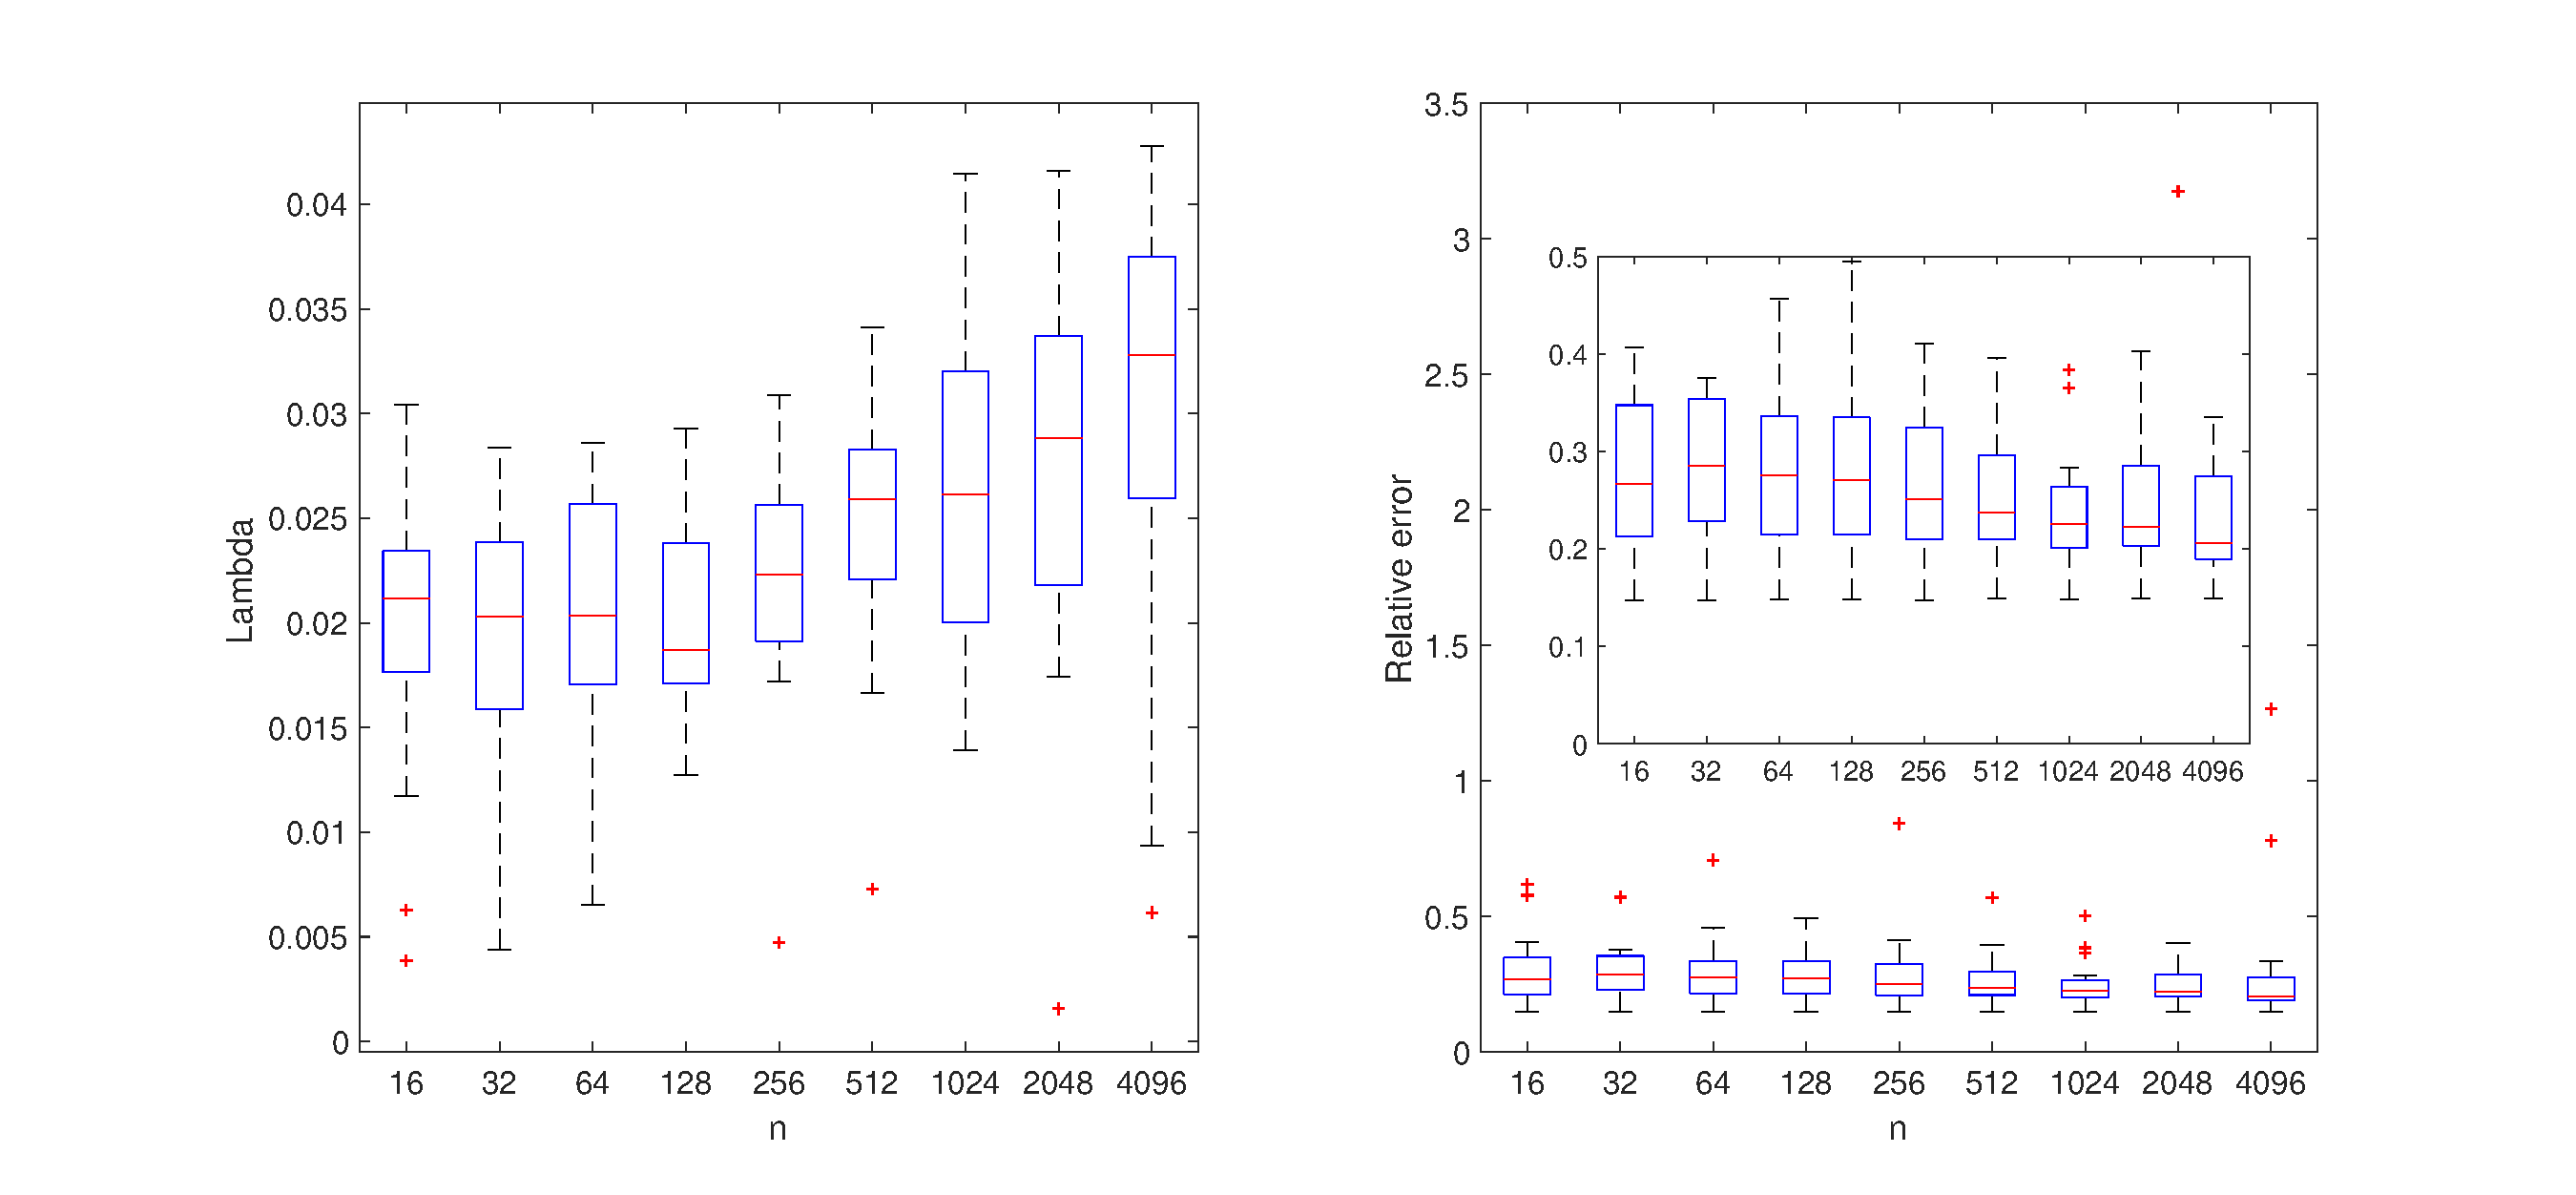
\includegraphics[scale = 0.4]{Figures/BothBoxes1D_F2_S05_W100_R20.eps}}
\caption{Box plots for the regularization parameters $\regparam_{\text{UPRE}}$ (left) and relative errors (right) across resolutions for 20 noise realizations. In this configuration, $\text{SNR = 5}$ and the width of the Gaussian kernel is 100.}
\label{BothBoxes1D_F2_S05_W100_R20}
\end{figure}

\begin{figure}
	\centerline{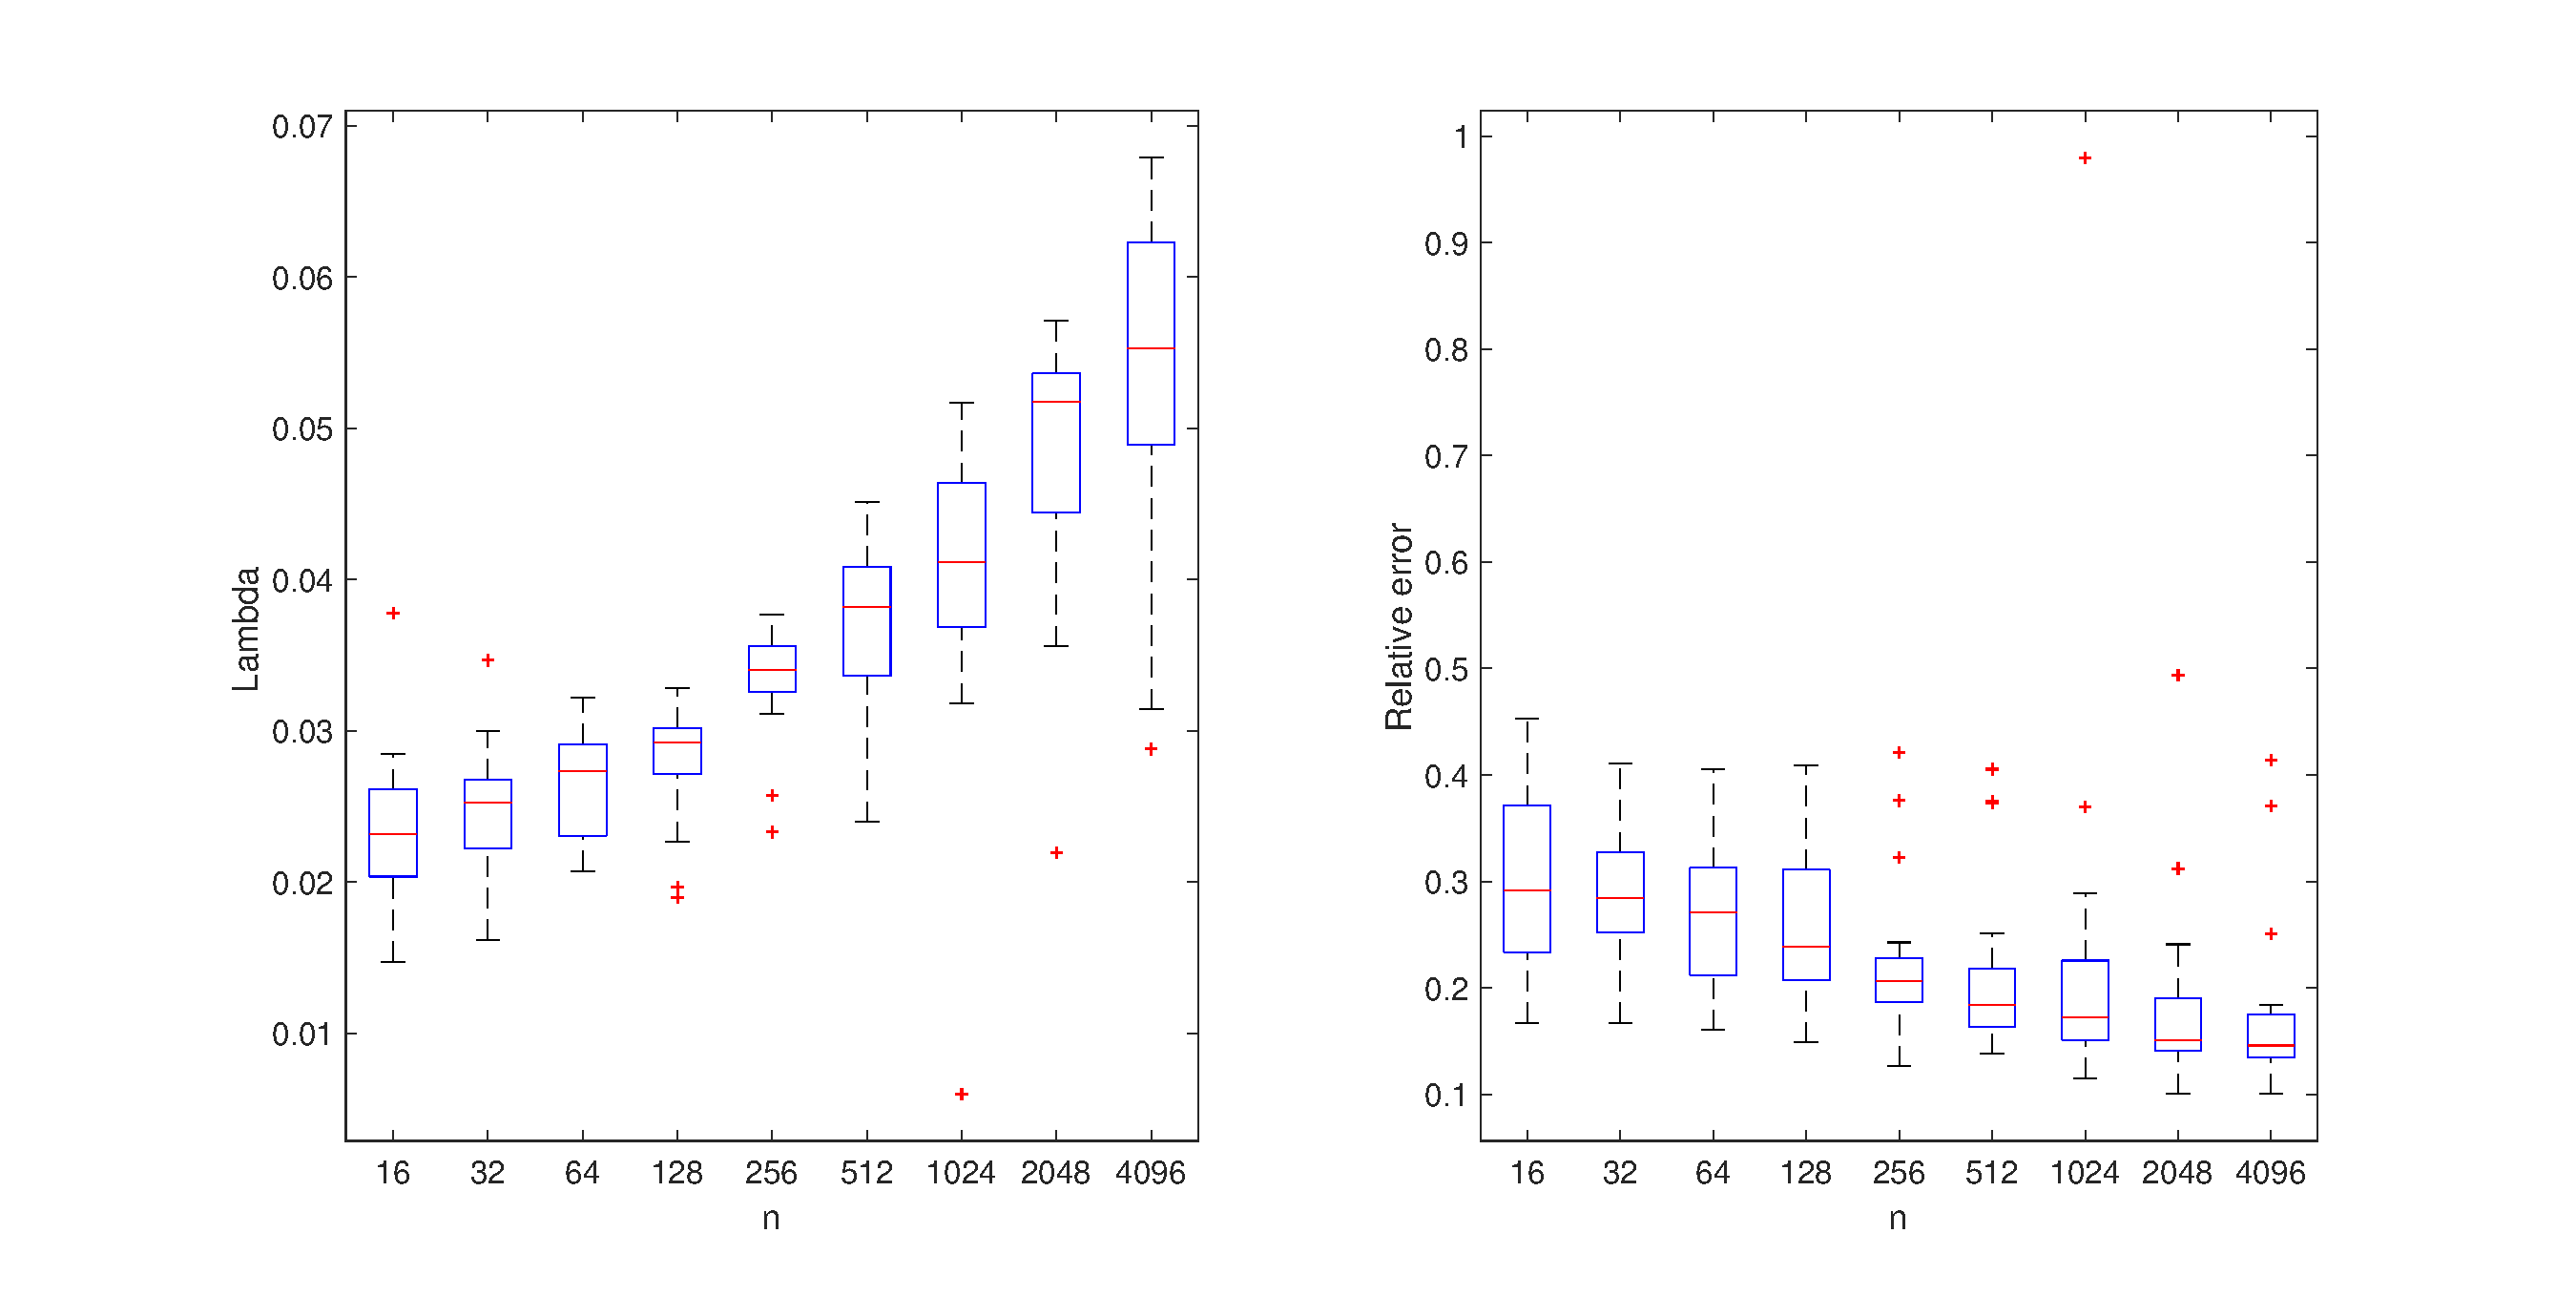
\includegraphics[scale = 0.4]{Figures/BothBoxes1D_F2_S05_W200_R20.eps}}
\caption{Box plots for the regularization parameters $\regparam_{\text{UPRE}}$  (left) and relative errors (right) across resolutions for 20 noise realizations. In this configuration, $\text{SNR = 5}$ and the width of the Gaussian kernel is 200.}
\end{figure}

\begin{figure}
	\centerline{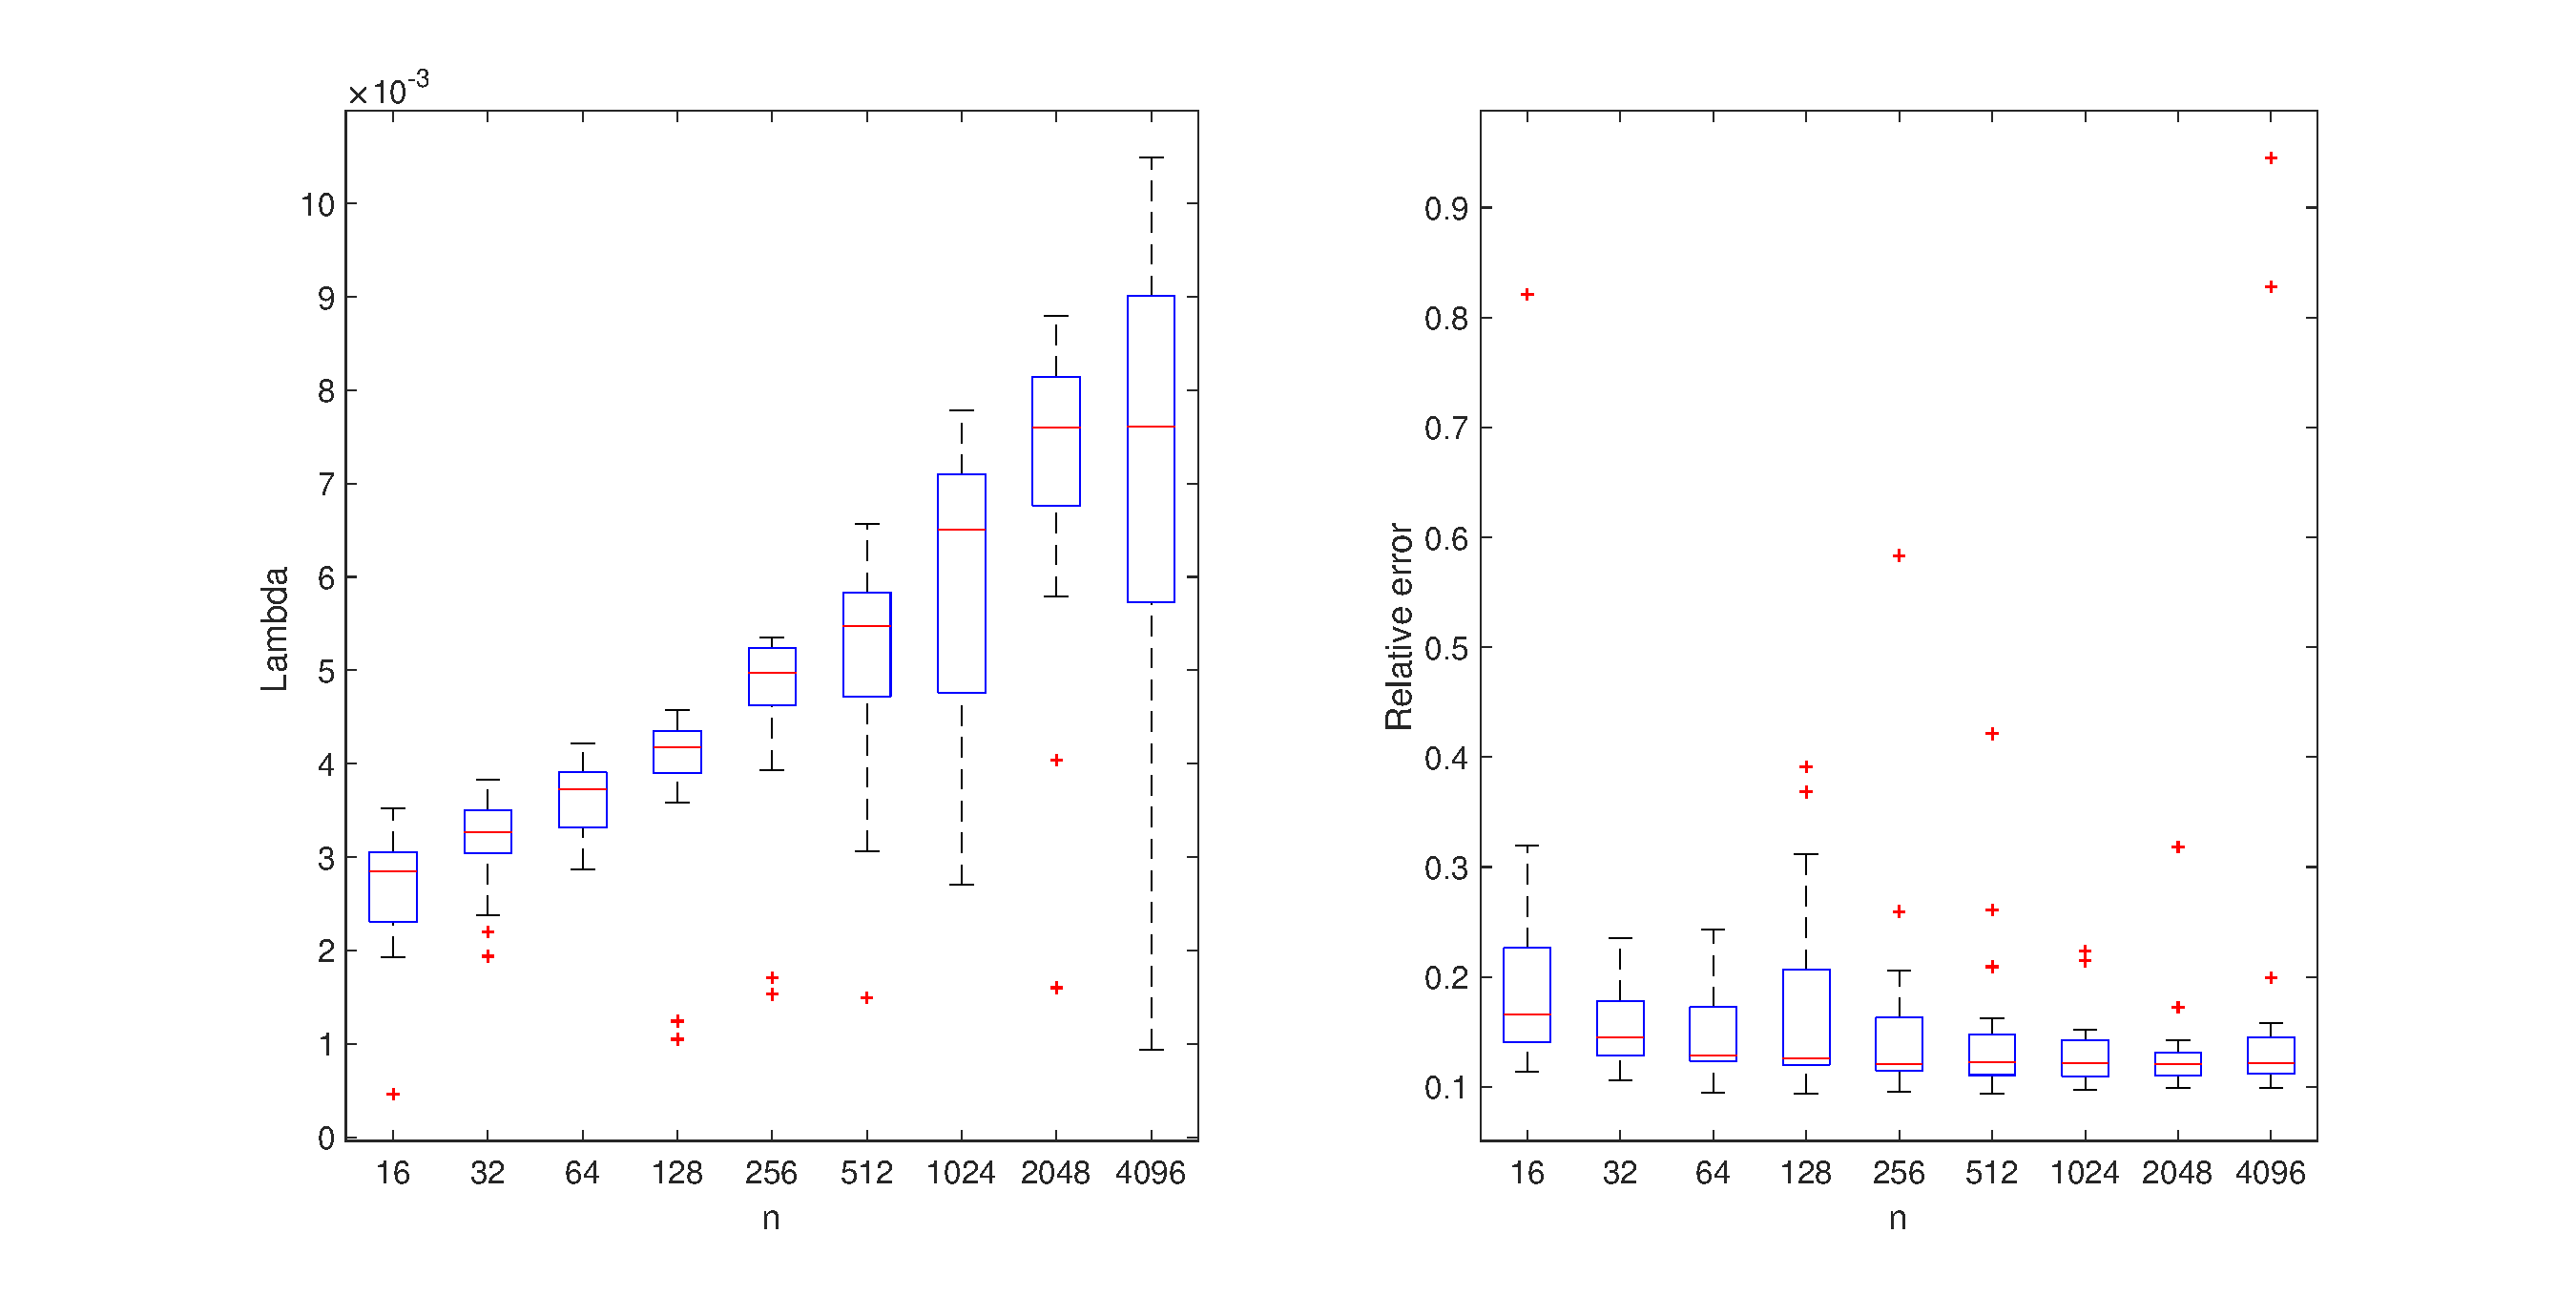
\includegraphics[scale = 0.4]{Figures/BothBoxes1D_F2_S25_W100_R20.eps}}
\caption{Box plots for the regularization parameters $\regparam_{\text{UPRE}}$  (left) and relative errors (right) across resolutions for 20 noise realizations. In this configuration, $\text{SNR = 25}$ and the width of the Gaussian kernel is 100.}
\end{figure}

\begin{figure}
	\centerline{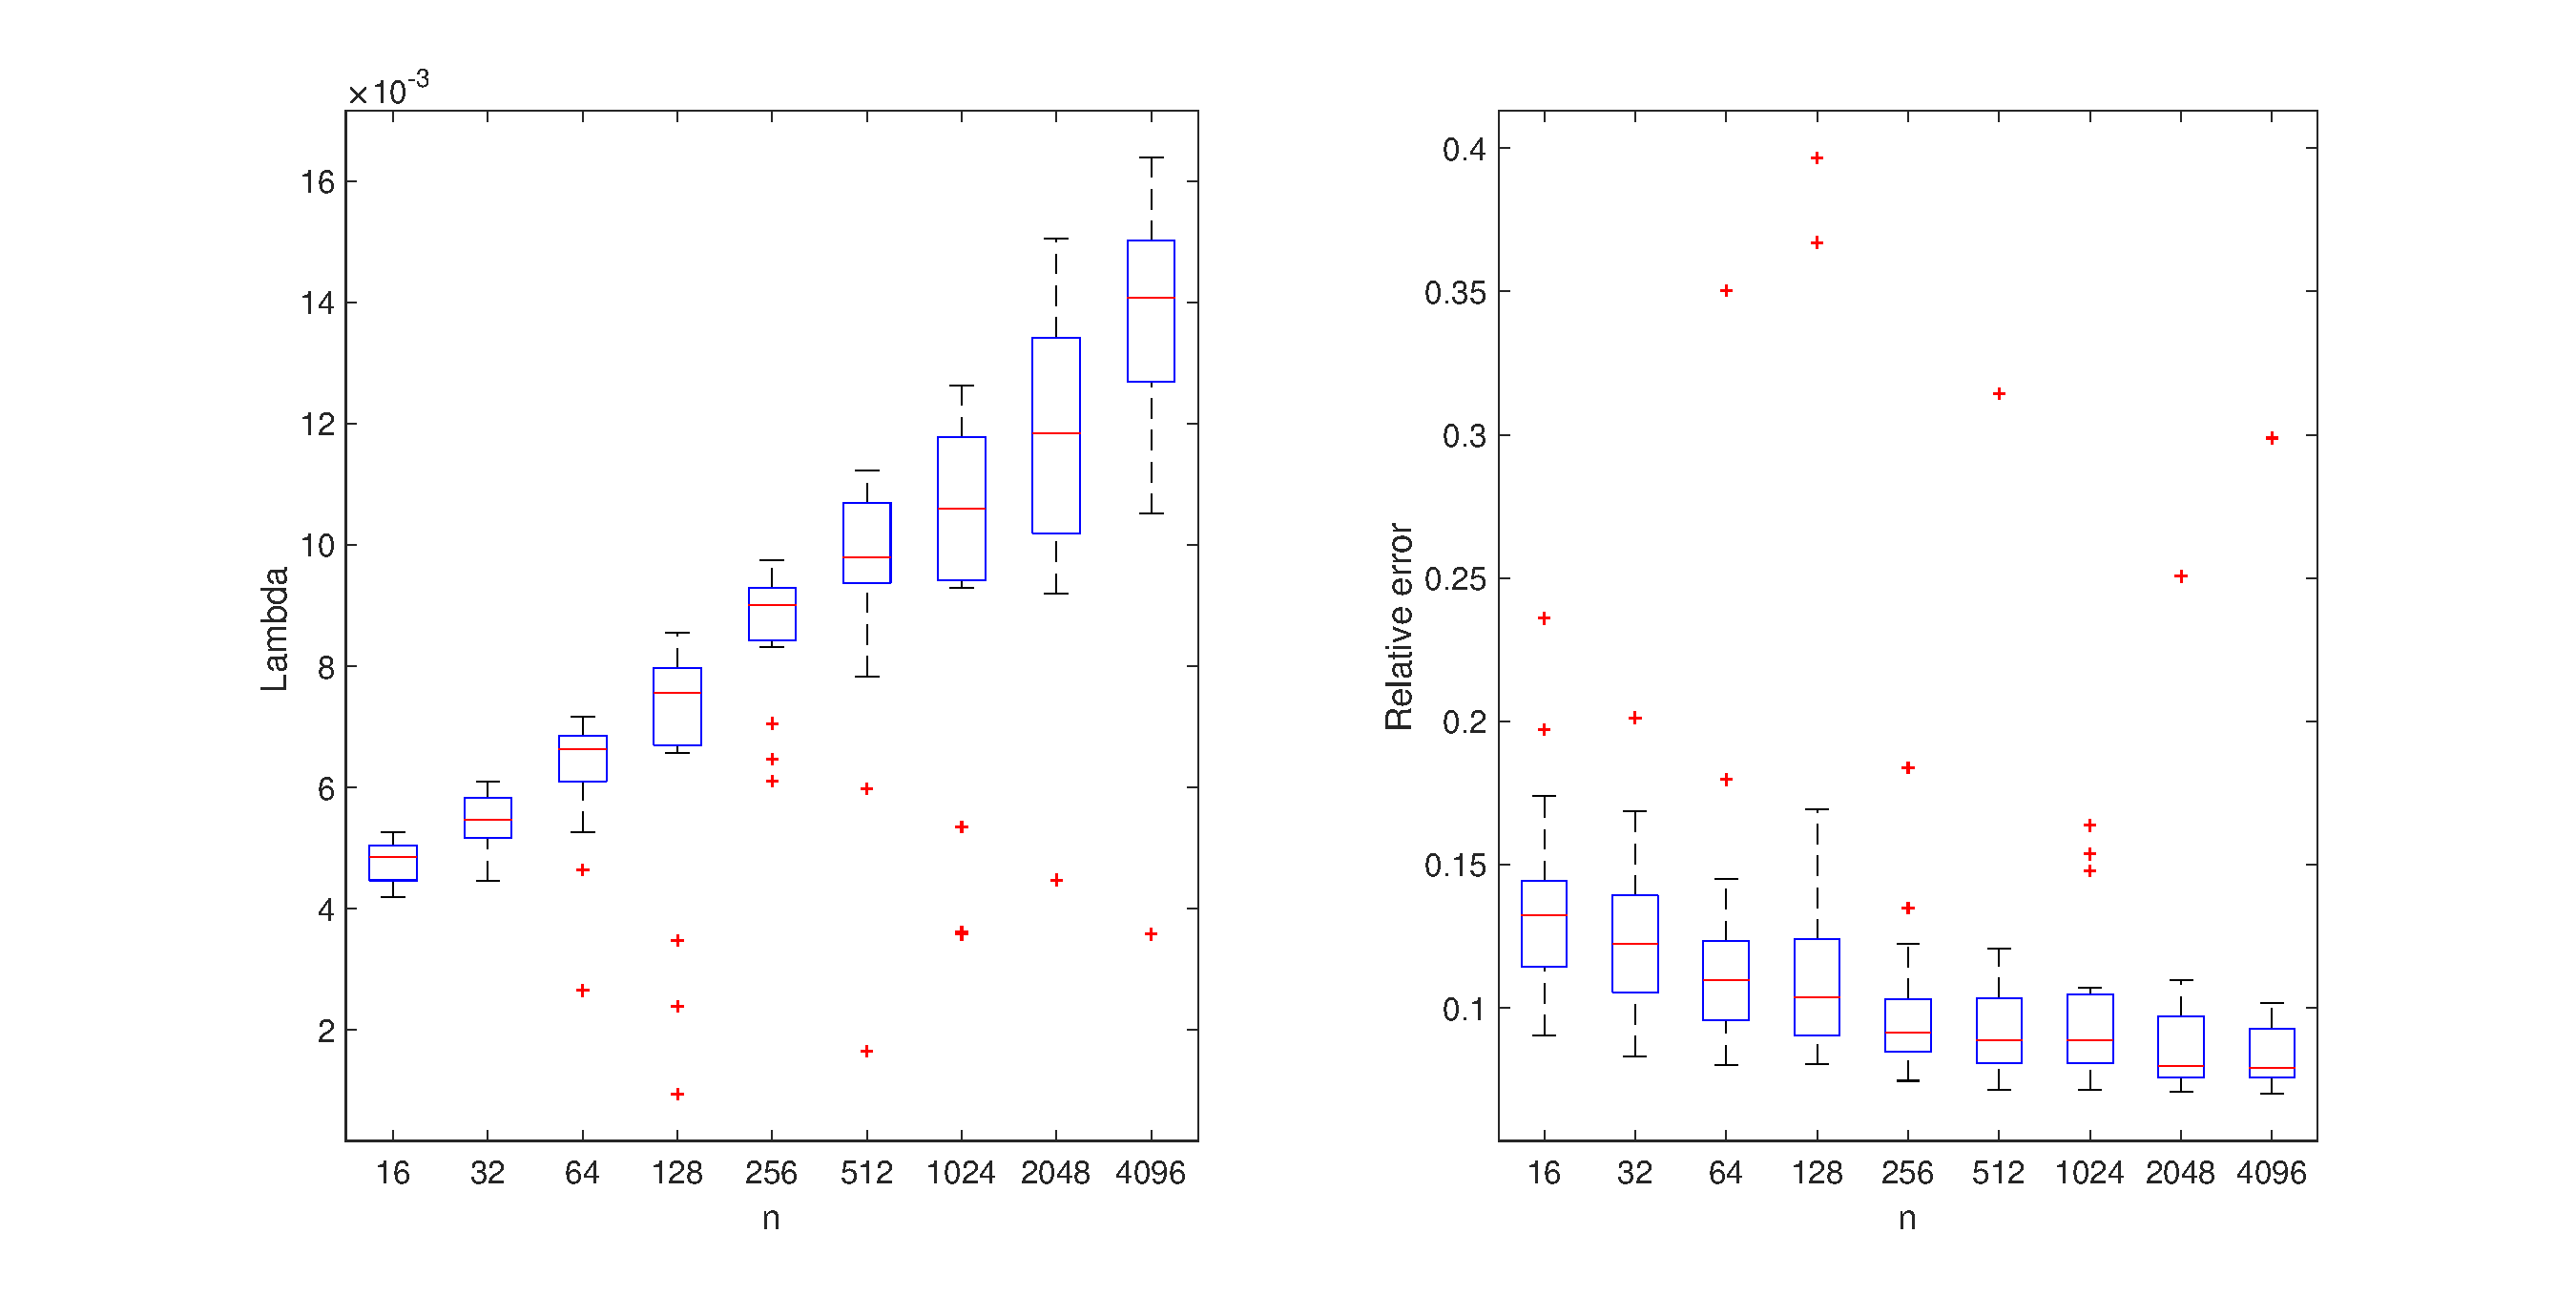
\includegraphics[scale = 0.4]{Figures/BothBoxes1D_F2_S25_W200_R20.eps}}
\caption{Box plots for the regularization parameters $\regparam_{\text{UPRE}}$  (left) and relative errors (right) across resolutions for 20 noise realizations. In this configuration, $\text{SNR = 25}$ and the width of the Gaussian kernel is 200.}
\label{BothBoxes1D_F2_S25_W200_R20}
\end{figure}

The relative errors are smaller for an SNR of 25 as opposed to an SNR of 5, which is to be expected since the variance in the noise is small for $\text{SNR} = 25$. Results pertaining to the Gaussian PSF of width 100 are poor compared to the results for the Gaussian PSF of width 200. In fact, the relative errors are exceedingly large for the width 100 Gaussian PSF; in Figure \ref{BothBoxes1D_F2_S05_W100_R20} there is an outlier with a relative error above 3. These outliers most likely arise from the difficulty in minimizing the often shallow graphs of the UPRE functionals. Figure \ref{BothBoxes1D_F2_S25_W200_R20} shows that the UPRE downsampling method performed the best for $\text{SNR} = 25$ and a Gaussian PSF of width 200. However, Figure \ref{BothBoxes1D_F2_S25_W200_R20} still shows numerous outliers, again which are probably a product of the functional minimization. 

\subsection{The GCV method} \label{The GCV method}
Of the 12 experimental configurations, four are presented here, all of which pertain to the second test function. The GCV method was used to select regularization parameters at each resolution. These parameters were used to construct regularized solutions of the full problem on $N = 4096$ points.

\subsection{The MDP method} \label{The MDP method}
Of the three methods considered in this report, the MDP method seemed to be the least robust with respect to downsampling. For many of the data configuration, finding a root of the MDP function proved unsuccesful; the components of the vectors representing the discretized MDP functions were often all positive, and so a root did not exist, at least in the $\regparam$ interval $[10^{-5},10]$. In MATLAB, the built-in function \texttt{fzero} was utilized to find roots of the MDP function. If no root could be found, \texttt{NaN} was returned. Since 20 noise realizations and 9 downsampling levels were considered, a total of 180 cases were tested for each data configuration. The safety parameter $\delta$ from \eqref{Eq_SpectralDP2} was set to 1.05.  \par 
Figure \ref{fig:MDPfailures} shows the sparsity of the resulting \texttt{NaN} cases for all data configurations considered. Perhaps the primary observation that can be made from Figure \ref{fig:MDPfailures} is that it is possible for root finding to fail at a certain downsampling level but succeed at a previous or subsequent level. This is evident from all of the plots, with the exception of the plots associated with the data configuration of an SNR of 25 and a width parameter of 100. For test functions \#1 and \#3, the MDP method for this data configuration failed considerably; no root of the MDP function was found for 110 cases ($\approx 61.1\%$) for test function \#1 and 112 cases ($\approx 62.2 \%$) for test function \#3. This data configuration proved somewhat more tractable is combination with test function \#2, with 40 cases ($\approx 22.2 \%$) of MDP method failure. This is somewhat surprising in light of the fact that test function \#2 is the least smooth of the three test functions.  \par 
One way of eliminating the number of failed cases would be to increase the value of $\delta$ in \eqref{Eq_SpectralDP2}. The result of doing so is actually twofold; not only does the number of failed cases decrease, but the consistency of the $\regparam_{\text{MDP}}$ improves. To emphasis this second result, Figure \ref{fig:MDPfunctions} shows that the tail ends of the functions fan out, while the curves appear to come together between $\lambda = 10^{-1}$ and $\lambda = 10^0$. Unfortunately the consistency of the $\regparam_{\text{MDP}}$ obtained by increasing $\delta$ yields regularized solutions with a greater amount of error, as shown in Figure 

\begin{figure}
	\centering
	\begin{subfigure}[b]{0.75\textwidth}
        \includegraphics[width=\textwidth]{Figures/MDPfailures1D_F1_R20.eps}
        \caption{}
        \label{fig:MDPfailure_F1}
    \end{subfigure}
    \vspace{-5pt}
    
    \begin{subfigure}[b]{0.75\textwidth}
        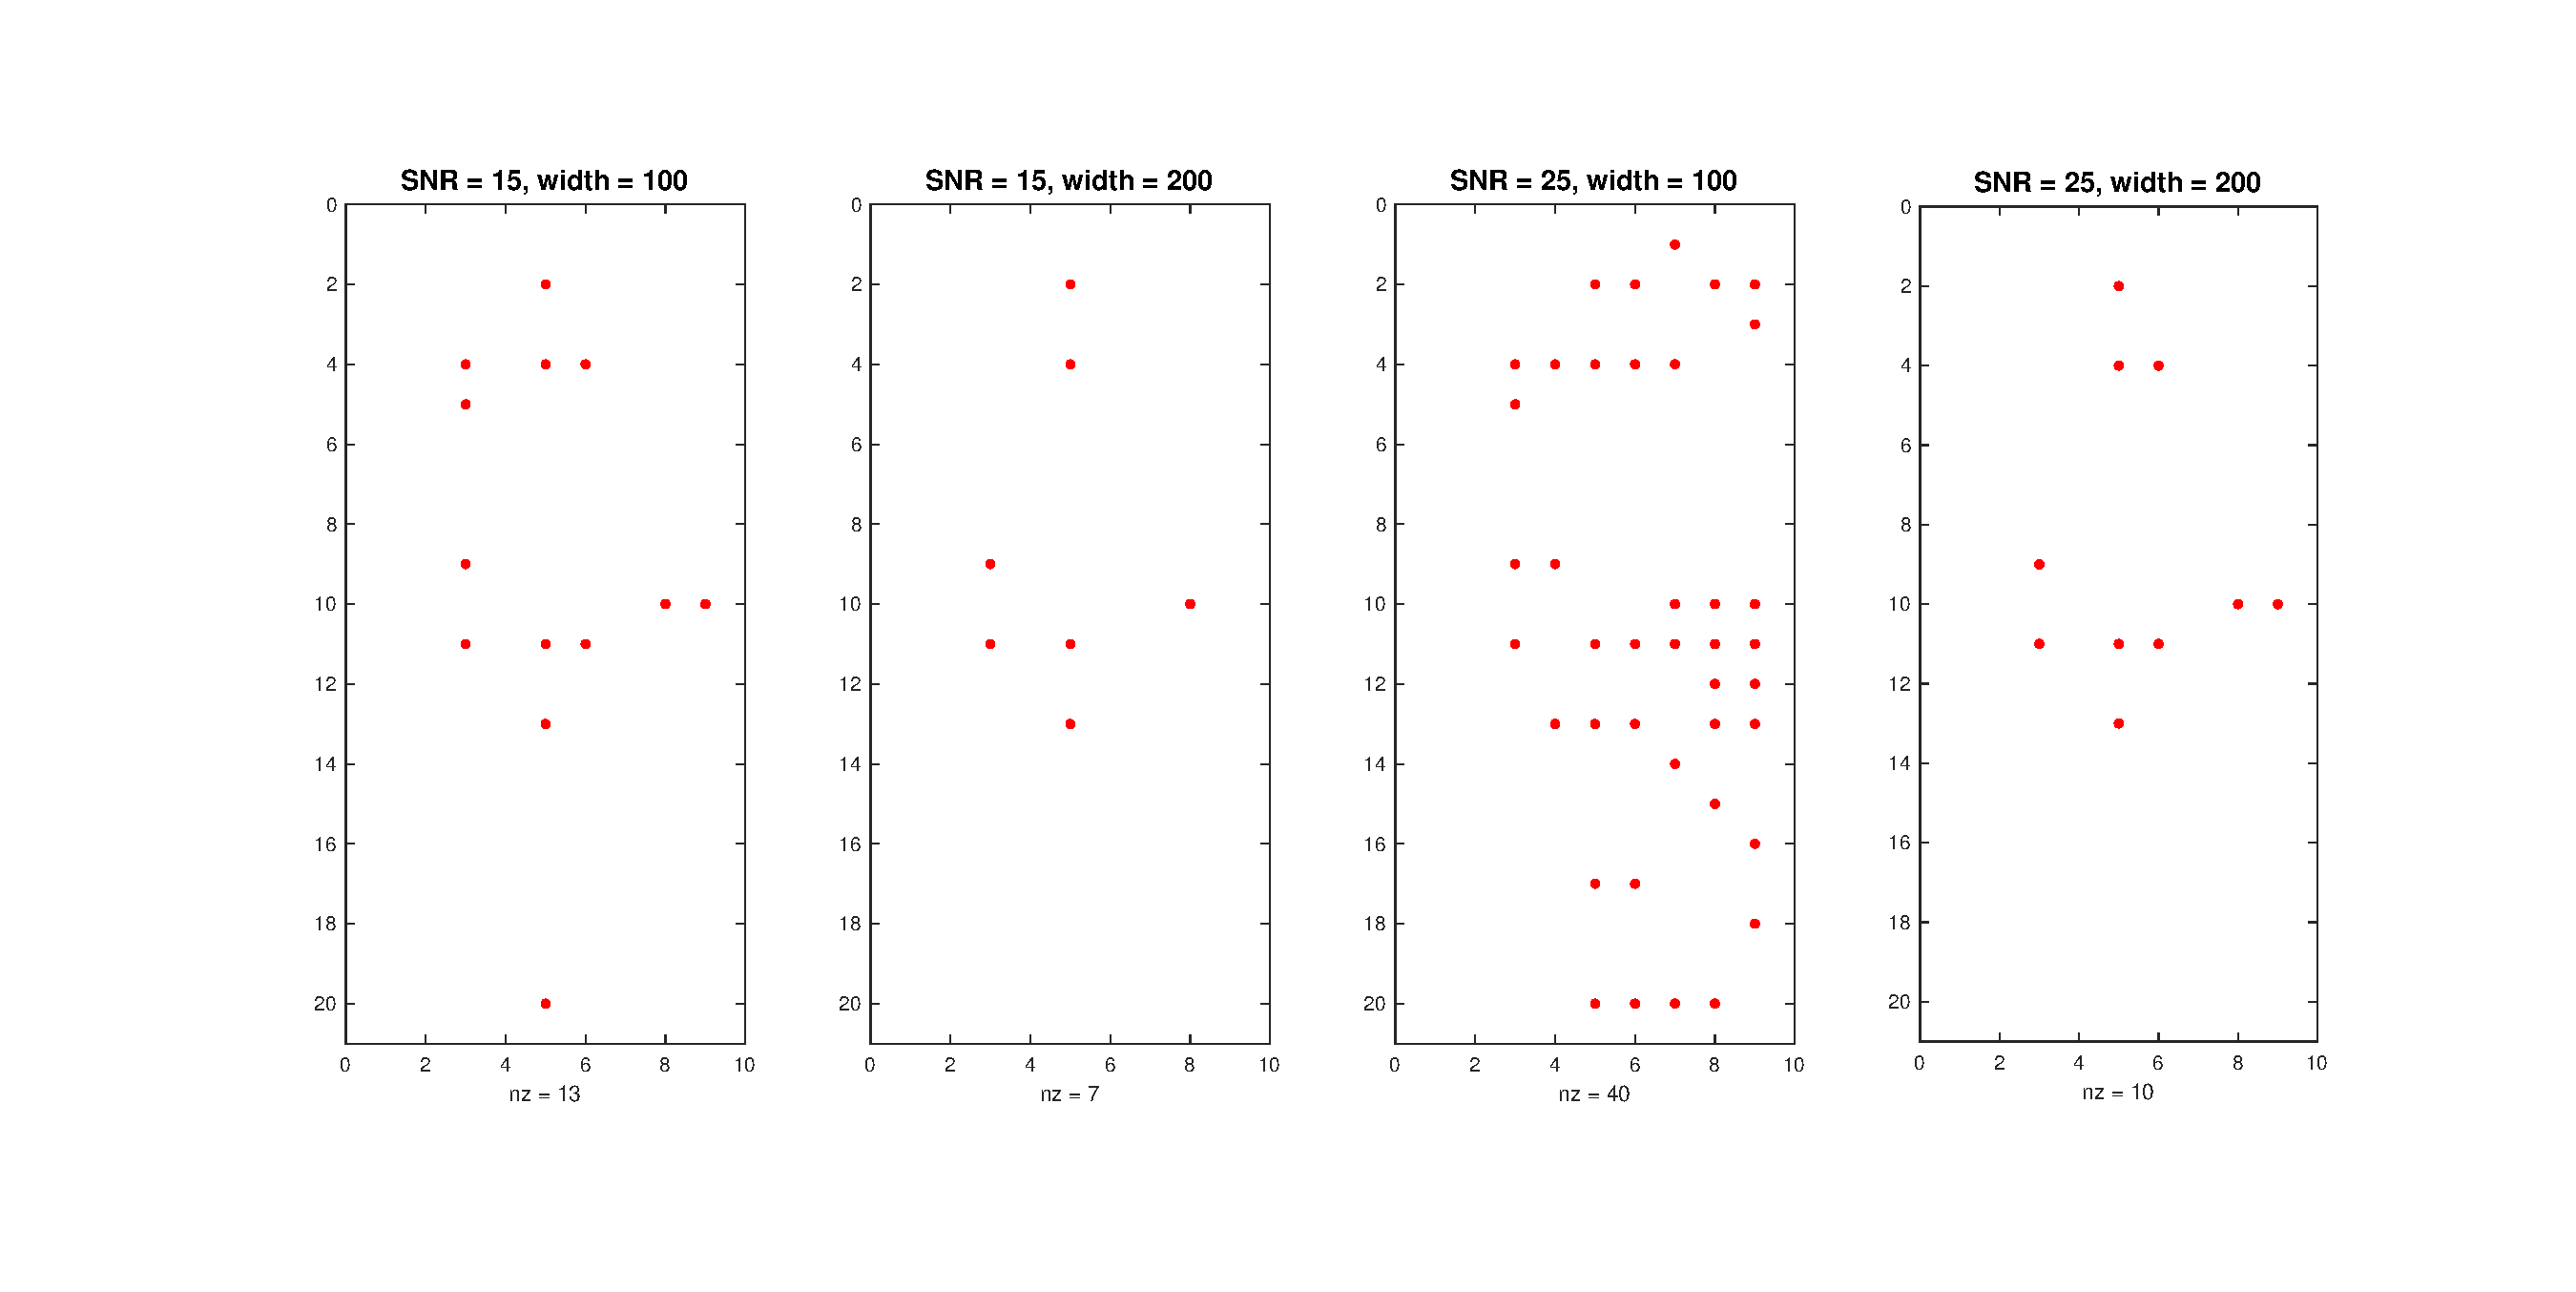
\includegraphics[width=\textwidth]{Figures/MDPfailures1D_F2_R20.eps}
        \caption{}
        \label{fig:MDPfailure_F2}
    \end{subfigure} 

    \begin{subfigure}[b]{0.75\textwidth}
        \includegraphics[width=\textwidth]{Figures/MDPfailures1D_F3_R20.eps}
        \caption{}
        \label{fig:MDPfailure_F3}
    \end{subfigure}
    \caption{The sparsity of MDP failures across noise realizations and downsampling levels. The rows represent noise realizations and the columns represent downsampling levels; the leftmost columns represent the $n = 16$ level and the rightmost represent the full $n = 4096$ level, with levels progressing by powers of 2 from left to right. The red dots represent \texttt{NaN}, which are the failures cases. The subfigures \ref{fig:MDPfailure_F1}, \ref{fig:MDPfailure_F2}, and \ref{fig:MDPfailure_F3} are the results for test functions \#1, \#2, and \#3, respectively.}
\label{fig:MDPfailures}
\end{figure}

\begin{figure}
	\centering
	\begin{subfigure}[b]{0.4\textwidth}
        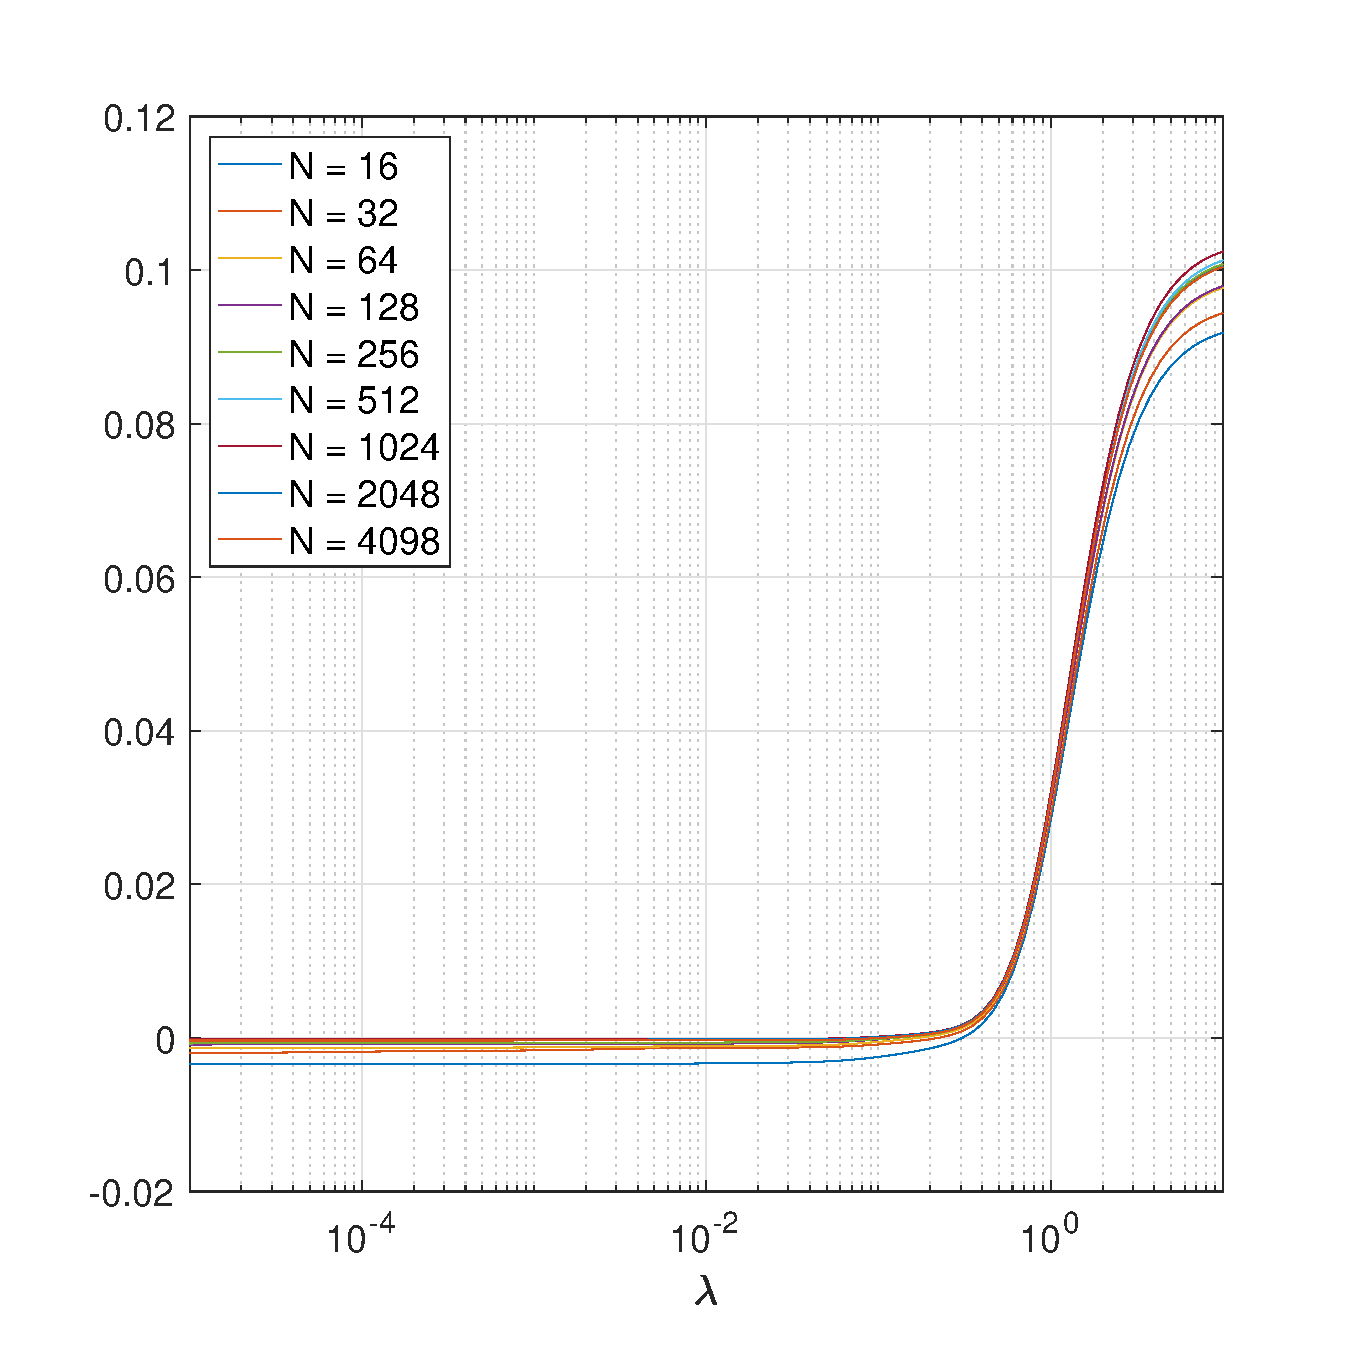
\includegraphics[width=\textwidth]{Figures/MDPfunctions_F1_S15_W100.eps}
        \caption{}
        \label{fig:MDPfunctions_notzoomed}
    \end{subfigure}
    \begin{subfigure}[b]{0.4\textwidth}
        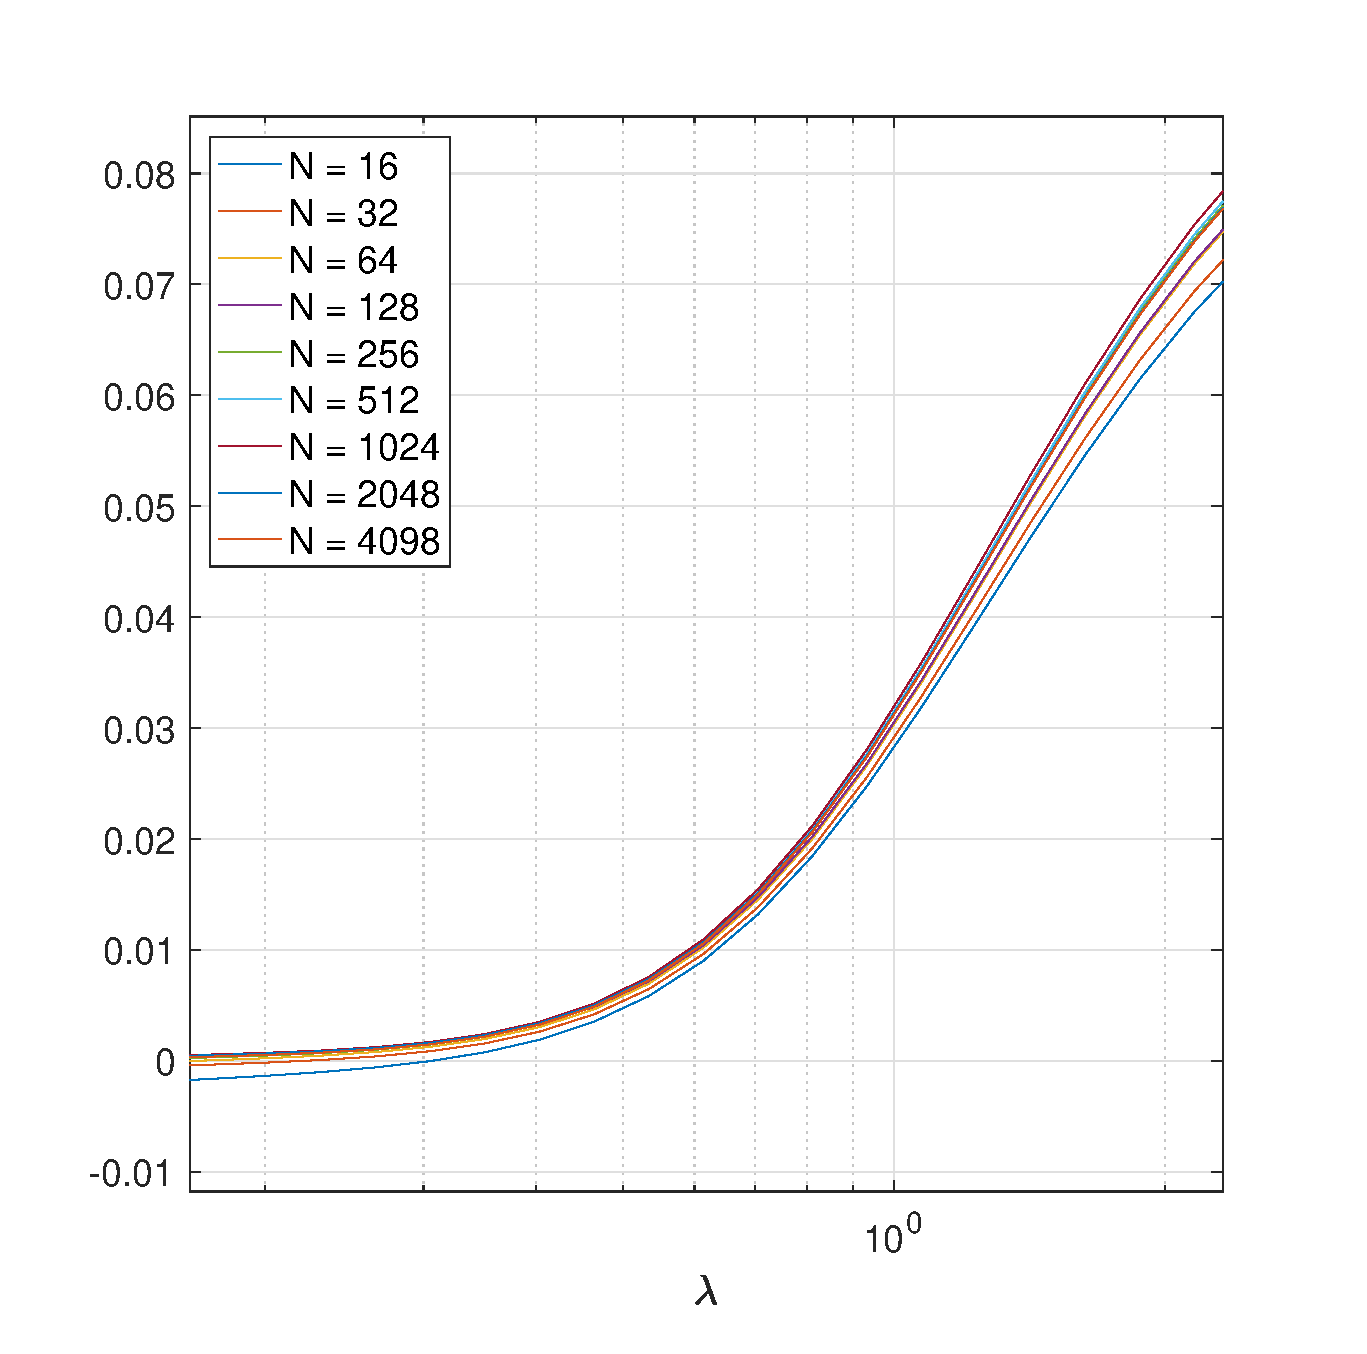
\includegraphics[width=\textwidth]{Figures/MDPfunctions_F1_S15_W100_zoomed.eps}
        \caption{}
        \label{fig:MDPfunctions_zoomed}
    \end{subfigure}
    \caption{}
\label{fig:MDPfunctions}
\end{figure}



\bibliographystyle{siam}
\bibliography{Parameter-Estimation}

\end{document}
